\documentclass[12pt]{article}

\usepackage{babel}

\newcommand{\pathtables}{./tables/}
\newcommand{\txline}{ \\ }

\newcommand{\sectionbreak}{\clearpage}

\usepackage{titlesec}
\titleformat{\section}
  {\normalfont\normalsize\bfseries}{\thesection.}{1em}{}
\titleformat{\subsection}
  {\normalfont\normalsize\bfseries\itshape}{\thesubsection.}{1em}{}
\titleformat{\subsubsection}
  {\normalfont\normalsize\itshape}{\thesubsubsection.}{1em}{}
\usepackage{geometry}
 \geometry{
 a4paper,
 left=25mm,
 top=25mm,
 bottom=20mm,
 right=25mm}

\usepackage{titling}
\usepackage[capposition=top]{floatrow}

\usepackage{amssymb}

\usepackage{graphicx}

\usepackage[normalem]{ulem}
\useunder{\uline}{\ul}{}

\usepackage{dcolumn}
\usepackage{booktabs}
\usepackage{float}
\usepackage{caption}
\usepackage[section]{placeins}
\usepackage{longtable}
\usepackage{multirow}
\usepackage{makecell}
\usepackage{lscape}
\usepackage{subcaption}
\usepackage{setspace}
\usepackage{tabularray}
\usepackage{subcaption}
\usepackage[capposition=top]{floatrow}

\usepackage{threeparttable}

\usepackage[hidelinks]{hyperref}  %hyperref still needs to be put at the end!

\usepackage{doi}

\title{Appendix -- Brand Transformation in European Politics: The Rise and Limits of Nonclassical Names}

\date{} 

\setcounter{secnumdepth}{0} % sections are level 1

\begin{document}
\sloppy

\begin{titlepage}
\begin{minipage}{\textwidth}
\maketitle
\thispagestyle{empty}
\setcounter{tocdepth}{2}
\tableofcontents
\vspace*{2cm}
\begin{center}
\textbf{The replication material for the empirical analysis is available at: \url{https://github.com/eborbath/party_brands}}
\end{center}
\end{minipage}
\end{titlepage}

\section{Appendix A: Additional figures and tables}

\subsection{Distributions of party brands}

\begin{figure}[H]
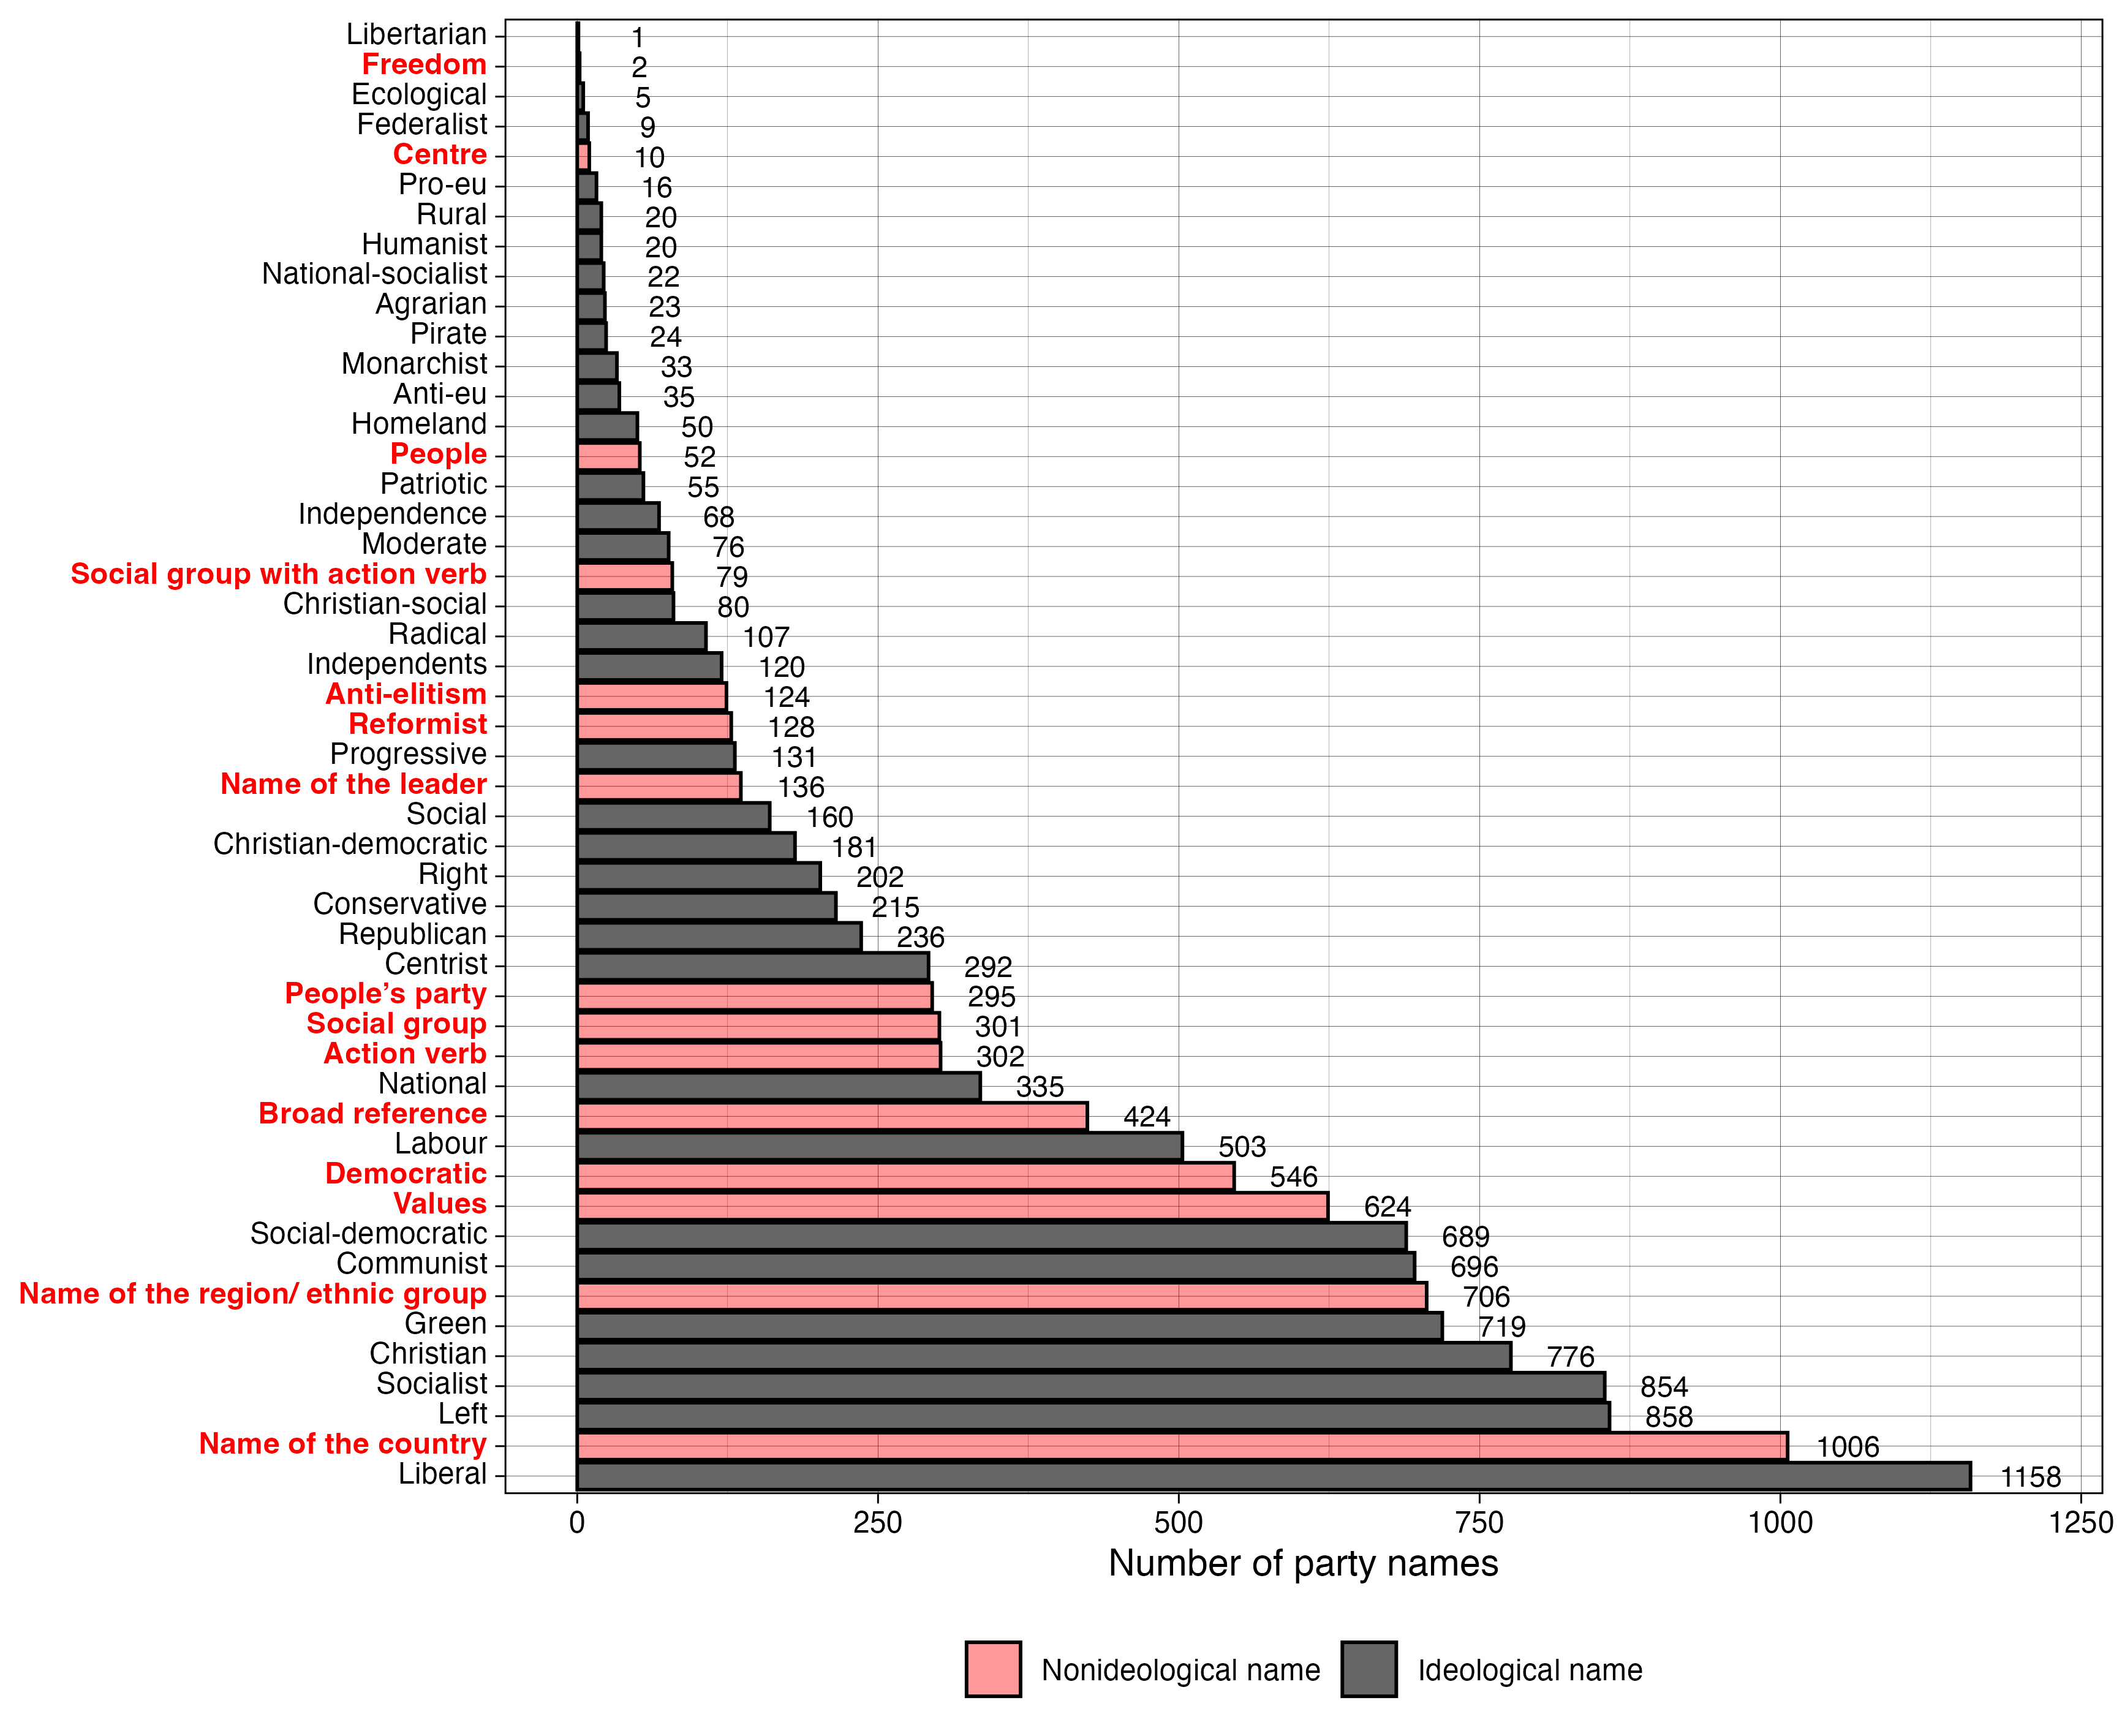
\includegraphics[width=\textwidth]{./Figures/ideology_types.png}
\caption{Programmatic references in the names of parties (1945-2023)}
\end{figure}

\clearpage

\begin{figure}[H]
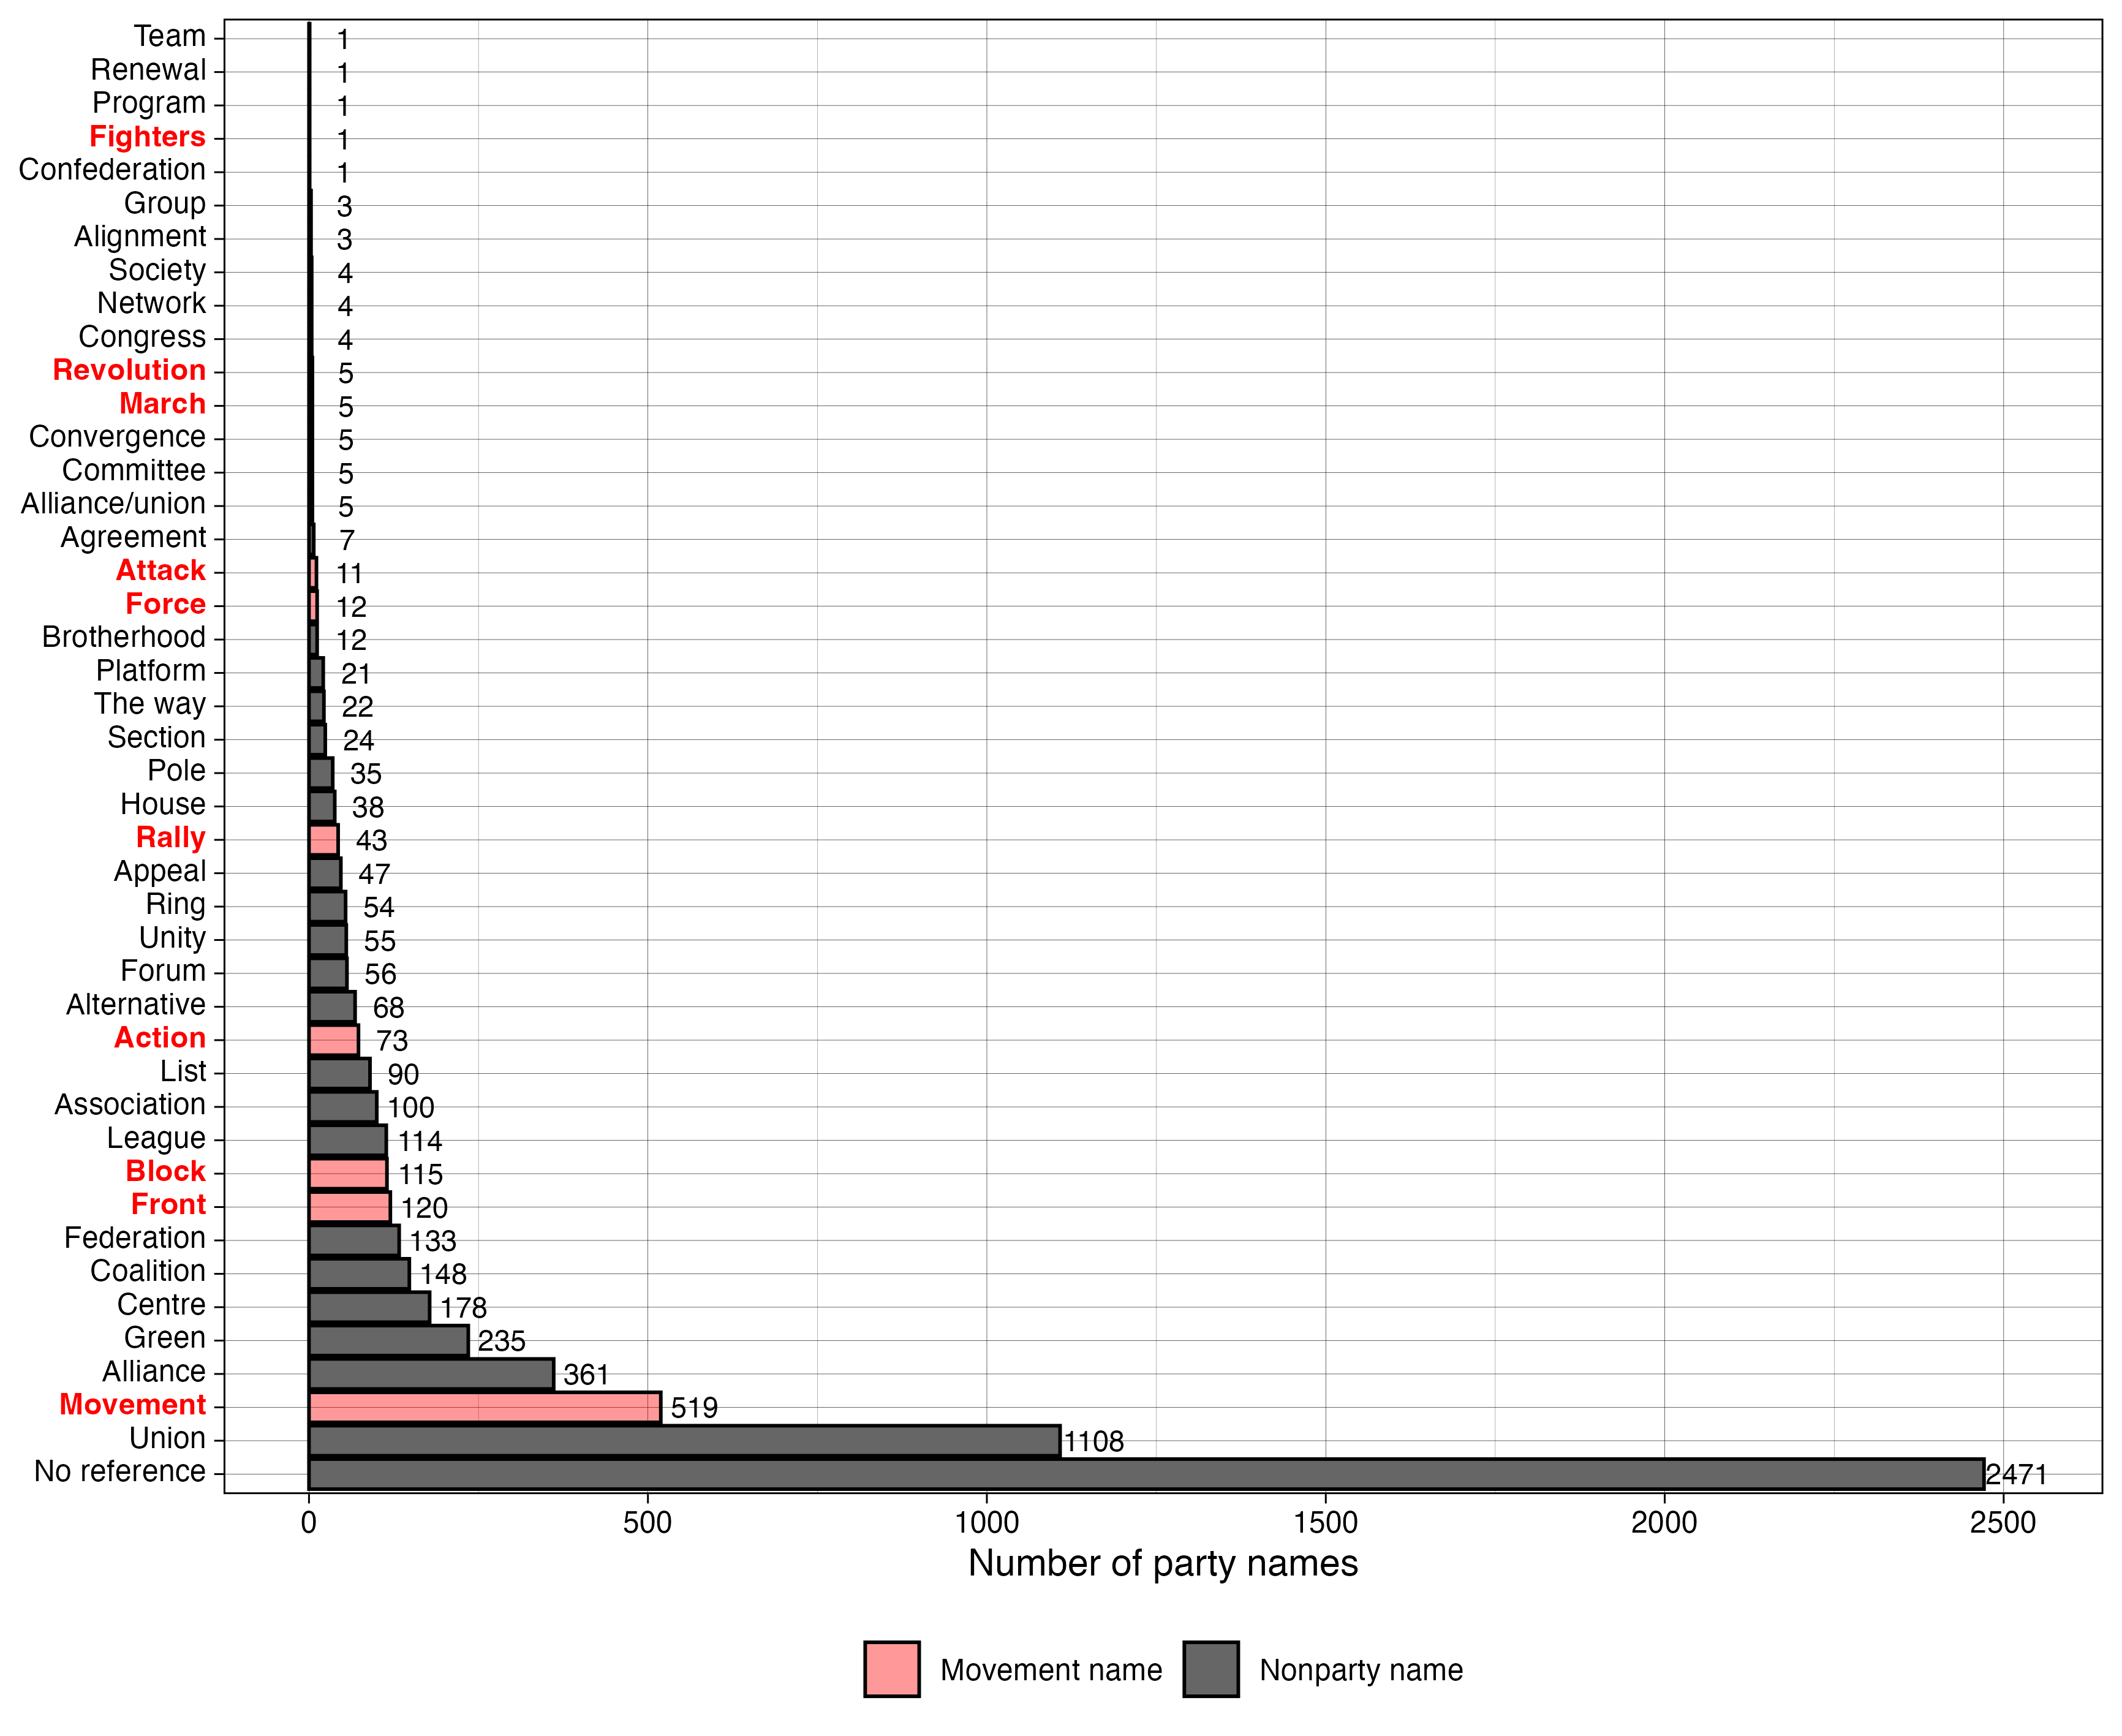
\includegraphics[width=\textwidth]{./Figures/org_types.png}
\caption{Organizational references in the names of parties (1945-2023)}
\end{figure}

\clearpage

\begin{figure}[H]
\caption{Distribution over time of party brands across 28 European countries (1945-2023)}
\label{Fig:timeline}
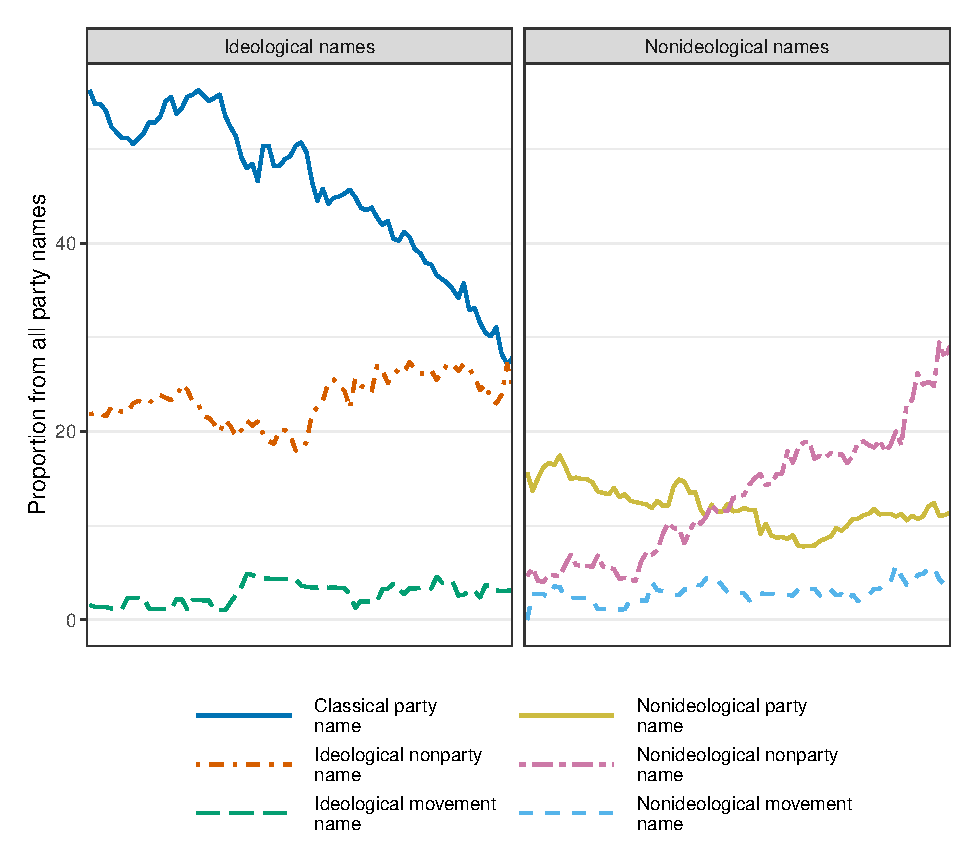
\includegraphics[width=\textwidth]{./Figures/all_types.eps}
\floatfoot{Note: The figure shows the average trend across all types.}
\end{figure}

\clearpage

\begin{table}[H]
\centering
\caption{\label{tab:unnamed-chunk-14}Distribution of brands by country \label{tab:country_table}}
\centering
\begin{tabular}[t]{l>{}lr>{}lr>{}lr}
\toprule
\multicolumn{1}{c}{ } & \multicolumn{2}{c}{\makecell[c]{Share of \\ classical \\ party \\ names}} & \multicolumn{2}{c}{\makecell[c]{Share of \\ nonideological \\ nonparty \\ names}} & \multicolumn{2}{c}{\makecell[c]{Share of \\ nonideological \\ movement \\ names}} \\
\cmidrule(l{3pt}r{3pt}){2-3} \cmidrule(l{3pt}r{3pt}){4-5} \cmidrule(l{3pt}r{3pt}){6-7}
  & Shape & t(`23)-t(0) & Shape & t(`23)-t(0) & Shape & t(`23)-t(0)\\
\midrule
AUT (1945-`21) & 
\includegraphics[width=0.67in, height=0.17in]{./figures/spec_plot/plot_16b67502bc200.pdf} & -33 & 
\includegraphics[width=0.67in, height=0.17in]{./figures/spec_plot/plot_16b676801e7c.pdf} & 17 & 
\includegraphics[width=0.67in, height=0.17in]{./figures/spec_plot/plot_16b67541f74f2.pdf} & 0\\
BEL (1945-`21) & 
\includegraphics[width=0.67in, height=0.17in]{./figures/spec_plot/plot_16b6719b14853.pdf} & -92 & 
\includegraphics[width=0.67in, height=0.17in]{./figures/spec_plot/plot_16b676207afbc.pdf} & 42 & 
\includegraphics[width=0.67in, height=0.17in]{./figures/spec_plot/plot_16b673f78a5c4.pdf} & 8\\
BGR (1990-`21) & 
\includegraphics[width=0.67in, height=0.17in]{./figures/spec_plot/plot_16b6730b0d67.pdf} & -20 & 
\includegraphics[width=0.67in, height=0.17in]{./figures/spec_plot/plot_16b673b1a0ff1.pdf} & 40 & 
\includegraphics[width=0.67in, height=0.17in]{./figures/spec_plot/plot_16b677053c52b.pdf} & -20\\
CHE (1945-`21) & 
\includegraphics[width=0.67in, height=0.17in]{./figures/spec_plot/plot_16b672f16d85.pdf} & -47 & 
\includegraphics[width=0.67in, height=0.17in]{./figures/spec_plot/plot_16b677661c8a8.pdf} & 36 & 
\includegraphics[width=0.67in, height=0.17in]{./figures/spec_plot/plot_16b674a40d3e7.pdf} & 9\\
CZE (1989-`21) & 
\includegraphics[width=0.67in, height=0.17in]{./figures/spec_plot/plot_16b6755a956e3.pdf} & -17 & 
\includegraphics[width=0.67in, height=0.17in]{./figures/spec_plot/plot_16b676586513b.pdf} & 9 & 
\includegraphics[width=0.67in, height=0.17in]{./figures/spec_plot/plot_16b6733e83387.pdf} & 14\\
DEU (1949-`21) & 
\includegraphics[width=0.67in, height=0.17in]{./figures/spec_plot/plot_16b675f20c31e.pdf} & -7 & 
\includegraphics[width=0.67in, height=0.17in]{./figures/spec_plot/plot_16b6726868c02.pdf} & 14 & 
\includegraphics[width=0.67in, height=0.17in]{./figures/spec_plot/plot_16b672f2fea5.pdf} & 0\\
DNK (1945-`21) & 
\includegraphics[width=0.67in, height=0.17in]{./figures/spec_plot/plot_16b671a3ca36.pdf} & -32 & 
\includegraphics[width=0.67in, height=0.17in]{./figures/spec_plot/plot_16b676f1f8e11.pdf} & 11 & 
\includegraphics[width=0.67in, height=0.17in]{./figures/spec_plot/plot_16b672c46ac7.pdf} & 0\\
ESP (1976-`21) & 
\includegraphics[width=0.67in, height=0.17in]{./figures/spec_plot/plot_16b67105cd0b4.pdf} & -10 & 
\includegraphics[width=0.67in, height=0.17in]{./figures/spec_plot/plot_16b6723b885b0.pdf} & 10 & 
\includegraphics[width=0.67in, height=0.17in]{./figures/spec_plot/plot_16b674dd0ca58.pdf} & 0\\
EST (1990-`21) & 
\includegraphics[width=0.67in, height=0.17in]{./figures/spec_plot/plot_16b6727483e40.pdf} & 43 & 
\includegraphics[width=0.67in, height=0.17in]{./figures/spec_plot/plot_16b6734d29458.pdf} & 14 & 
\includegraphics[width=0.67in, height=0.17in]{./figures/spec_plot/plot_16b673f32c30a.pdf} & 0\\
FIN (1945-`21) & 
\includegraphics[width=0.67in, height=0.17in]{./figures/spec_plot/plot_16b6767c7e0e6.pdf} & -11 & 
\includegraphics[width=0.67in, height=0.17in]{./figures/spec_plot/plot_16b67785c51c5.pdf} & 33 & 
\includegraphics[width=0.67in, height=0.17in]{./figures/spec_plot/plot_16b6731a5fec3.pdf} & 0\\
FRA (1945-`21) & 
\includegraphics[width=0.67in, height=0.17in]{./figures/spec_plot/plot_16b676a098298.pdf} & -50 & 
\includegraphics[width=0.67in, height=0.17in]{./figures/spec_plot/plot_16b6773f29872.pdf} & 29 & 
\includegraphics[width=0.67in, height=0.17in]{./figures/spec_plot/plot_16b67686dbce.pdf} & 0\\
GBR (1945-`21) & 
\includegraphics[width=0.67in, height=0.17in]{./figures/spec_plot/plot_16b67338d0a25.pdf} & -6 & 
\includegraphics[width=0.67in, height=0.17in]{./figures/spec_plot/plot_16b673c77b95b.pdf} & 11 & 
\includegraphics[width=0.67in, height=0.17in]{./figures/spec_plot/plot_16b6751d160e0.pdf} & 0\\
GRC (1974-`21) & 
\includegraphics[width=0.67in, height=0.17in]{./figures/spec_plot/plot_16b674dc8d7a3.pdf} & -14 & 
\includegraphics[width=0.67in, height=0.17in]{./figures/spec_plot/plot_16b6736ba47d8.pdf} & 19 & 
\includegraphics[width=0.67in, height=0.17in]{./figures/spec_plot/plot_16b677c120eb6.pdf} & 0\\
HRV (1991-`21) & 
\includegraphics[width=0.67in, height=0.17in]{./figures/spec_plot/plot_16b67376b3901.pdf} & -33 & 
\includegraphics[width=0.67in, height=0.17in]{./figures/spec_plot/plot_16b674f6773f6.pdf} & 50 & 
\includegraphics[width=0.67in, height=0.17in]{./figures/spec_plot/plot_16b6720cafe7f.pdf} & 22\\
HUN (1989-`21) & 
\includegraphics[width=0.67in, height=0.17in]{./figures/spec_plot/plot_16b6734fb0bd9.pdf} & -7 & 
\includegraphics[width=0.67in, height=0.17in]{./figures/spec_plot/plot_16b67abfba9b.pdf} & 2 & 
\includegraphics[width=0.67in, height=0.17in]{./figures/spec_plot/plot_16b67f3c9dda.pdf} & 27\\
IRL (1945-`21) & 
\includegraphics[width=0.67in, height=0.17in]{./figures/spec_plot/plot_16b673f635ee1.pdf} & -11 & 
\includegraphics[width=0.67in, height=0.17in]{./figures/spec_plot/plot_16b673dc1bebd.pdf} & 17 & \includegraphics[width=0.67in, height=0.17in]{./figures/spec_plot/plot_16b672a111251.pdf} & 0\\
ITA (1945-`21) & \includegraphics[width=0.67in, height=0.17in]{./figures/spec_plot/plot_16b671877cf00.pdf} & -60 & \includegraphics[width=0.67in, height=0.17in]{./figures/spec_plot/plot_16b6752b8f61f.pdf} & 20 & \includegraphics[width=0.67in, height=0.17in]{./figures/spec_plot/plot_16b675d772274.pdf} & 20\\
LTU (1990-`21) & \includegraphics[width=0.67in, height=0.17in]{./figures/spec_plot/plot_16b673ae7cc72.pdf} & 0 & \includegraphics[width=0.67in, height=0.17in]{./figures/spec_plot/plot_16b67ae4b46.pdf} & 17 & \includegraphics[width=0.67in, height=0.17in]{./figures/spec_plot/plot_16b67143909ba.pdf} & 0\\
LUX (1945-`21) & \includegraphics[width=0.67in, height=0.17in]{./figures/spec_plot/plot_16b67794db8a.pdf} & -25 & \includegraphics[width=0.67in, height=0.17in]{./figures/spec_plot/plot_16b676dbda604.pdf} & 0 & \includegraphics[width=0.67in, height=0.17in]{./figures/spec_plot/plot_16b673a0b45fd.pdf} & 0\\
LVA (1990-`21) & \includegraphics[width=0.67in, height=0.17in]{./figures/spec_plot/plot_16b6733b3cb8.pdf} & -50 & \includegraphics[width=0.67in, height=0.17in]{./figures/spec_plot/plot_16b675ced921e.pdf} & 46 & \includegraphics[width=0.67in, height=0.17in]{./figures/spec_plot/plot_16b67b98c380.pdf} & -25\\
NLD (1945-`21) & \includegraphics[width=0.67in, height=0.17in]{./figures/spec_plot/plot_16b6738c2a955.pdf} & 5 & \includegraphics[width=0.67in, height=0.17in]{./figures/spec_plot/plot_16b67600e947c.pdf} & 38 & \includegraphics[width=0.67in, height=0.17in]{./figures/spec_plot/plot_16b6775a18cad.pdf} & 12\\
NOR (1945-`21) & \includegraphics[width=0.67in, height=0.17in]{./figures/spec_plot/plot_16b676e23ffc5.pdf} & 17 & \includegraphics[width=0.67in, height=0.17in]{./figures/spec_plot/plot_16b6727a877e7.pdf} & 0 & \includegraphics[width=0.67in, height=0.17in]{./figures/spec_plot/plot_16b674f0bb2b4.pdf} & 0\\
POL (1989-`21) & \includegraphics[width=0.67in, height=0.17in]{./figures/spec_plot/plot_16b675014155.pdf} & -17 & \includegraphics[width=0.67in, height=0.17in]{./figures/spec_plot/plot_16b673114a55f.pdf} & 33 & \includegraphics[width=0.67in, height=0.17in]{./figures/spec_plot/plot_16b673d5dc5bf.pdf} & 0\\
PRT (1974-`21) & \includegraphics[width=0.67in, height=0.17in]{./figures/spec_plot/plot_16b676cb24b96.pdf} & -28 & \includegraphics[width=0.67in, height=0.17in]{./figures/spec_plot/plot_16b6715c5ee39.pdf} & 44 & \includegraphics[width=0.67in, height=0.17in]{./figures/spec_plot/plot_16b6749d0dc8f.pdf} & -17\\
ROU (1989-`21) & \includegraphics[width=0.67in, height=0.17in]{./figures/spec_plot/plot_16b6756a959cc.pdf} & 0 & \includegraphics[width=0.67in, height=0.17in]{./figures/spec_plot/plot_16b67dd15c61.pdf} & 11 & \includegraphics[width=0.67in, height=0.17in]{./figures/spec_plot/plot_16b6728d7af5f.pdf} & 0\\
SVK (1993-`21) & \includegraphics[width=0.67in, height=0.17in]{./figures/spec_plot/plot_16b674fb3f74f.pdf} & -26 & \includegraphics[width=0.67in, height=0.17in]{./figures/spec_plot/plot_16b673bed3d40.pdf} & 29 & \includegraphics[width=0.67in, height=0.17in]{./figures/spec_plot/plot_16b675f90efc2.pdf} & -8\\
SVN (1989-`21) & \includegraphics[width=0.67in, height=0.17in]{./figures/spec_plot/plot_16b674f99bde.pdf} & 12 & \includegraphics[width=0.67in, height=0.17in]{./figures/spec_plot/plot_16b6765991d22.pdf} & 0 & \includegraphics[width=0.67in, height=0.17in]{./figures/spec_plot/plot_16b676681b9ec.pdf} & 12\\
SWE (1945-`21) & \includegraphics[width=0.67in, height=0.17in]{./figures/spec_plot/plot_16b6768878f14.pdf} & -10 & \includegraphics[width=0.67in, height=0.17in]{./figures/spec_plot/plot_16b675d874f6b.pdf} & 12 & \includegraphics[width=0.67in, height=0.17in]{./figures/spec_plot/plot_16b671d034680.pdf} & 0\\
\bottomrule
\multicolumn{7}{l}{\rule{0pt}{1em}Note: The values represent the share of parties from all parties in a country/year context.}\\
\end{tabular}
\end{table}


\newpage

\begin{figure}[H]
\includegraphics[width=\textwidth]{./Figures/country_timeline.eps}
\caption{Over time distribution of party brands within countries (1945-2023)}
\end{figure}

\newpage

\subsection{Correlational analysis}

\begin{figure}[H]
\centering
\includegraphics[width=\textwidth]{./Figures/corplot_party.png}
\caption{Correlation between party level predictors}
\floatfoot{Note: Missing values are excluded pairwise.}
\end{figure}

\clearpage

\begin{figure}[H]
\centering
\includegraphics[width=\textwidth]{./Figures/corplot_context.png}
\caption{Correlation between context level predictors}
\floatfoot{Note: For the purposes of the plot, the dependent variables have been averaged at the country*year level. Missing values are excluded pairwise.}
\end{figure}

\clearpage


\begin{table}[h!]
\caption{Hierarchical logistic regression models of party brands (1945-2023)}
\begin{center}
\begin{tabular}{l@{} D{)}{)}{9)3}@{} D{)}{)}{9)3}@{} D{)}{)}{11)3}@{}}
\toprule
 & \multicolumn{1}{c}{Classical} & \multicolumn{1}{c}{Nonideological} & \multicolumn{1}{c}{Nonideological} \\
 & \multicolumn{1}{c}{party name} & \multicolumn{1}{c}{nonparty name} & \multicolumn{1}{c}{movement name} \\
\midrule
Intercept                        & -0.77 \; (0.27)^{**}  & -3.14 \; (0.28)^{***} & -7.86 \;  (0.80)^{***} \\
Party family (ref: Christ. dem.) &                       &                       &                        \\
\quad Communist/Socialist        & 1.74 \; (0.09)^{***}  & -0.66 \; (0.13)^{***} & -0.97 \;  (0.37)^{**}  \\
\quad Social democracy           & 1.62 \; (0.08)^{***}  & -0.87 \; (0.12)^{***} & -0.20 \;  (0.28)       \\
\quad Green/Ecologist            & 1.11 \; (0.10)^{***}  & -0.57 \; (0.14)^{***} & -0.45 \;  (0.36)       \\
\quad Liberal                    & 0.10 \; (0.08)        & 0.27 \; (0.11)^{*}    & 0.92 \;  (0.25)^{***}  \\
\quad Conservative               & 0.02 \; (0.09)        & 0.81 \; (0.10)^{***}  & 0.91 \;  (0.27)^{***}  \\
\quad Agrarian                   & 0.23 \; (0.14)        & 1.28 \; (0.16)^{***}  & 0.64 \;  (0.50)        \\
\quad Right-wing                 & -0.06 \; (0.10)       & 0.66 \; (0.11)^{***}  & 1.74 \;  (0.25)^{***}  \\
\quad Other                      & -3.01 \; (0.46)^{***} & 1.00 \; (0.16)^{***}  & -1.71 \;  (1.05)       \\
Gov. status                      &                       &                       &                        \\
\quad Past PM party              & -0.04 \; (0.08)       & 0.17 \; (0.12)        & -12.20 \; (48.38)      \\
\quad Opp. party                 & -0.32 \; (0.06)^{***} & 0.27 \; (0.08)^{***}  & 0.79 \;  (0.18)^{***}  \\
Party features                   &                       &                       &                        \\
\quad Log(party age)             & 2.30 \; (0.14)^{***}  & -2.10 \; (0.13)^{***} & -1.33 \;  (0.25)^{***} \\
\quad Vote share                 & 0.22 \; (0.11)^{*}    & 0.17 \; (0.15)        & 1.23 \;  (0.31)^{***}  \\
\quad Electoral coalition        & -1.90 \; (0.17)^{***} & 1.01 \; (0.11)^{***}  & -1.59 \;  (0.30)^{***} \\
System features                  &                       &                       &                        \\
\quad Econ. polariz.             & -0.10 \; (0.08)       & 0.07 \; (0.10)        & -0.32 \;  (0.22)       \\
\quad Cult. polariz.             & -0.10 \; (0.09)       & 0.05 \; (0.11)        & -0.06 \;  (0.21)       \\
\quad Electoral volatil.         & -0.27 \; (0.08)^{**}  & 0.28 \; (0.09)^{**}   & -0.08 \;  (0.20)       \\
\quad Turnout                    & 0.10 \; (0.10)        & -0.18 \; (0.11)       & 0.31 \;  (0.26)        \\
\quad Electoral dem.             & 0.64 \; (0.18)^{***}  & 0.40 \; (0.25)        & -0.54 \;  (0.50)       \\
\quad Presidentialism            & 0.41 \; (0.25)        & -0.01 \; (0.32)       & 2.31 \;  (0.72)^{**}   \\
Decades (ref: 1945-1969)         &                       &                       &                        \\
\quad 1970-1989                  & -0.27 \; (0.08)^{***} & 0.68 \; (0.14)^{***}  & 0.66 \;  (0.25)^{**}   \\
\quad 1990-2008                  & -0.43 \; (0.09)^{***} & 0.86 \; (0.15)^{***}  & 0.83 \;  (0.27)^{**}   \\
\quad 2009-2023                  & -0.95 \; (0.10)^{***} & 1.33 \; (0.16)^{***}  & 1.09 \;  (0.29)^{***}  \\
\midrule
AIC                              & 12418.33              & 9061.05               & 2650.03                \\
BIC                              & 12602.88              & 9245.60               & 2834.58                \\
Num. obs.                        & 11874                 & 11874                 & 11874                  \\
Country*Year                     & 1398                  & 1398                  & 1398                   \\
Country                          & 27                    & 27                    & 27                     \\
\bottomrule
\multicolumn{4}{l}{\scriptsize{$^{***}p<0.001$; $^{**}p<0.01$; $^{*}p<0.05$}}
\end{tabular}
\label{table:mlm_reg_table_all}
\end{center}
\end{table}



\clearpage

\subsection{The effect of party organizations}

In this part of the appendix, we examine the effect of two organizational features on party brands. We rely on the VParty dataset and select two items. First, regarding candidate nominations, we rely on the item \textit{v2panom}: 

\begin{itemize}
  \item[]{Question: Which of the following options best describes the process by which the party decides on candidates for the national legislative elections?}
  \item[]{Clarification: If nomination procedures vary across constituencies consider the most common practice.}
  \item[]{Responses}
  \begin{enumerate}
  \item{The party leader unilaterally decides on which candidates will run for the party in national legislative elections.}
  \item{The national party leadership (i.e. an executive committee) collectively decides which candidates will run for the party in national legislative elections.}
  \item{Delegates of local/regional organizations decide which candidates will run for the party in national legislative elections.}
  \item{All party members decide on which candidates will run for the party in national legislative elections in primaries/caucuses.}
  \item{All registered voters decide on which candidates will run for the party in national legislative elections in primaries/caucuses.}
  \end{enumerate}
\end{itemize}

Second, concerning internal cohesion, we rely on the item \textit{v2padisa}:

\begin{itemize}
  \item[]{Question: To what extent do the elites in this party display disagreement over party strategies?}
  \item[]{Clarification: Party strategies include election campaign strategy, policy stance, distribution of party financial resources, cooperation with other parties (i.e. coalition formation), and the selection of legislative and presidential candidates as well as the party leader. Party elites are prominent and influential party members such as current and former ministers, members of parliament or the party leadership, regional and municipal leaders, and opinion leaders. They do not necessarily have to be the part of the official party leadership.}
  \item[]{Responses}
  \begin{enumerate}
  \item{Party elites display almost complete disagreement over party strategies and many party elites have left the party.}
  \item{Party elites display a high level of visible disagreement over party strategies and some of them have left the party.}
  \item{Party elites display some visible disagreement over party strategies, but none of them have left the party.}
  \item{Party elites display negligible visible disagreement over party strategies.}
  \item{Party elites display virtually no visible disagreement over party strategies.}
  \end{enumerate}
\end{itemize}

Both of these variables are coded at election dates. Therefore, we carry their values forward to the next election. Despite this filling strategy, both items are missing in a substantial part of our dataset. Figure \ref{Fig:missings} shows the country*year combinations where the two variables are observed.

\begin{figure}[H]
\includegraphics[width=\textwidth]{./Figures/missing_map.png}
\caption{Coverage of the VParty variables}
\label{Fig:missings} 
\floatfoot{Note: This figure visualizes the availability of the VParty variables. Each row represents a country, and each column corresponds to a year. Cells filled in gray indicate years for which data is available. Empty cells outlined in black denote years where data is expected but missing. Cells with no frame are years for which no observations exist in the dataset, typically due to countries entering the dataset later.}
\end{figure}

In what follows, we replicate the multilevel regression analysis using the same specification as presented in the paper on this partial sample, and present the marginal effect of the first lag of the two organizational variables.

\clearpage


\begin{table}[h!]
\caption{Partial sample (1970-2023) - hierarchical logistic regression models of party brands with additional independent variables}
\begin{center}
\begin{tabular}{l@{} D{)}{)}{12)3}@{} D{)}{)}{9)3}@{} D{)}{)}{16)3}@{}}
\toprule
 & \multicolumn{1}{c}{Classical} & \multicolumn{1}{c}{Nonideological} & \multicolumn{1}{c}{Nonideological} \\
 & \multicolumn{1}{c}{party name} & \multicolumn{1}{c}{nonparty name} & \multicolumn{1}{c}{movement name} \\
\midrule
Intercept                        & -0.90 \;   (0.36)^{*}   & -4.06 \; (0.64)^{***} & -12.32 \;       (2.33)^{***} \\
Party family (ref: Christ. dem.) &                         &                       &                              \\
\quad Right-wing                 & -0.47 \;   (0.17)^{**}  & 0.71 \; (0.23)^{**}   & 1.69 \;       (0.49)^{***}   \\
\quad Green/Ecologist            & 0.62 \;   (0.19)^{***}  & -1.15 \; (0.31)^{***} & 0.47 \;       (0.67)         \\
\quad Communist/Socialist        & 2.78 \;   (0.21)^{***}  & -2.22 \; (0.34)^{***} & -46.89 \; (3592291.85)       \\
\quad Conservative               & 0.00 \;   (0.15)        & 1.61 \; (0.22)^{***}  & 3.90 \;       (0.64)^{***}   \\
\quad Social democracy           & 2.62 \;   (0.14)^{***}  & -2.47 \; (0.25)^{***} & -2.32 \;       (0.73)^{**}   \\
\quad Liberal                    & 0.08 \;   (0.13)        & 0.45 \; (0.19)^{*}    & -0.63 \;       (0.49)        \\
\quad Agrarian                   & 0.27 \;   (0.22)        & 1.99 \; (0.31)^{***}  & -52.92 \; (4774555.68)       \\
\quad Other                      & -15.70 \; (128.01)      & 0.51 \; (0.60)        & -6.57 \;       (7.09)        \\
Party features                   &                         &                       &                              \\
\quad Candidate nomination       & -1.65 \;   (0.17)^{***} & 1.38 \; (0.24)^{***}  & -4.01 \;       (0.62)^{***}  \\
\quad Internal cohesion          & -0.64 \;   (0.17)^{***} & -0.28 \; (0.22)       & 2.14 \;       (0.53)^{***}   \\
\quad Past PM party              & 0.12 \;   (0.13)        & -0.42 \; (0.27)       & -27.55 \;  (333460.41)       \\
\quad Opp. party                 & -0.22 \;   (0.09)^{**}  & 0.43 \; (0.13)^{***}  & 0.49 \;       (0.34)         \\
\quad Log(party age)             & 2.49 \;   (0.34)^{***}  & -2.54 \; (0.41)^{***} & 0.61 \;       (0.96)         \\
\quad Vote share                 & -1.06 \;   (0.20)^{***} & 1.06 \; (0.28)^{***}  & 1.01 \;       (0.60)         \\
\quad Electoral coalition        & -2.18 \;   (0.26)^{***} & 1.25 \; (0.21)^{***}  & -3.08 \;       (0.57)^{***}  \\
System features                  &                         &                       &                              \\
\quad Econ. polariz.             & 0.09 \;   (0.16)        & 0.09 \; (0.21)        & -2.45 \;       (0.53)^{***}  \\
\quad Cult. polariz.             & 0.24 \;   (0.16)        & 0.20 \; (0.22)        & -0.56 \;       (0.46)        \\
\quad Electoral volatil.         & -0.27 \;   (0.14)^{*}   & 0.50 \; (0.19)^{**}   & -0.49 \;       (0.46)        \\
\quad Turnout                    & -0.17 \;   (0.15)       & -0.13 \; (0.22)       & -0.13 \;       (0.55)        \\
\quad Electoral dem.             & 0.42 \;   (0.47)        & 1.77 \; (0.69)^{*}    & -3.95 \;       (1.04)^{***}  \\
\quad Presidentialism            & 0.51 \;   (0.45)        & 1.08 \; (1.05)        & -1.03 \;       (4.65)        \\
Decades (ref: 1970-1989)         &                         &                       &                              \\
\quad 1990-2008                  & -0.34 \;   (0.11)^{**}  & 0.18 \; (0.19)        & 0.00 \;       (0.43)         \\
\quad 2009-2023                  & -0.81 \;   (0.13)^{***} & 0.81 \; (0.21)^{***}  & 0.00 \;       (0.48)         \\
\midrule
AIC                              & 4645.52                 & 2375.36               & 616.78                       \\
BIC                              & 4812.87                 & 2542.71               & 784.13                       \\
Num. obs.                        & 4612                    & 4612                  & 4612                         \\
Country*Year                     & 974                     & 974                   & 974                          \\
Country                          & 27                      & 27                    & 27                           \\
\bottomrule
\multicolumn{4}{l}{\scriptsize{$^{***}p<0.001$; $^{**}p<0.01$; $^{*}p<0.05$}}
\end{tabular}
\label{table:mlm_reg_table_partial}
\end{center}
\end{table}



\clearpage

\begin{figure}[H] 
\includegraphics[width=\textwidth]{./Figures/logit_partial_sample.png} 
\caption{Logistic regression model of party naming} 
\floatfoot{\textit{Note:} Estimates are from the partial sample shown above. Thick error bars represent 90\% confidence intervals; thin error bars represent 95\% confidence intervals. The model is a three-level logistic regression with random intercepts, nesting observations within country*years and countries.} 
\label{Fig:mlm_results_partial} 
\end{figure}

\clearpage

\section{Appendix B: Re-branding parties}

\setcounter{figure}{0}
\setcounter{table}{0}

\subsection{Distributions of re-branding parties}

\begin{figure}[H]
\includegraphics[width=\textwidth]{./Figures/rebranded_parties.png}
\caption{Number of parties re-branding between 1945-2023}
\end{figure}

\clearpage

\begin{figure}[H]
\includegraphics[width=\textwidth]{./Figures/re_branding_timeline.eps}
\caption{Distribution over time of re-branding parties across 28 European countries (1945-2023)}
\label{Fig:re_branding_timeline}
\floatfoot{Note: The figure shows the average trend across all countries.}
\end{figure}

\clearpage

\begin{figure}[H]
\includegraphics[width=\textwidth]{./Figures/re_branding_families.eps}
\caption{Distribution over party families of re-branding parties across 28 European countries (1945-2023)}
\label{Fig:re_branding_families}
\floatfoot{Note: The figure shows the average shares within party families.}
\end{figure}

\clearpage

\subsection{Correlational analysis}


\begin{table}[h!]
\caption{Overall re-branding (1945-2023) - hierarchical logistic regression models}
\begin{center}
\begin{tabular}{l@{} D{)}{)}{9)3}@{} D{)}{)}{9)3}@{} D{)}{)}{9)3}@{}}
\toprule
 & \multicolumn{1}{c}{Classical} & \multicolumn{1}{c}{Nonideological} & \multicolumn{1}{c}{Nonideological} \\
 & \multicolumn{1}{c}{party name} & \multicolumn{1}{c}{nonparty name} & \multicolumn{1}{c}{movement name} \\
\midrule
Intercept                          & -5.74 \; (2.18)^{**} & -4.92 \; (2.51)^{*}  & -5.31 \; (2.24)^{*}  \\
Party family (ref: Christ. dem.)   &                      &                      &                      \\
\quad Right-wing                   & -0.02 \; (0.45)      & 0.65 \; (0.50)       & -0.75 \; (0.52)      \\
\quad Green/Ecologist              & -0.21 \; (0.55)      & 0.27 \; (0.61)       & -0.63 \; (0.61)      \\
\quad Communist/Socialist          & -0.57 \; (0.48)      & -0.21 \; (0.56)      & -0.37 \; (0.50)      \\
\quad Conservative                 & -0.31 \; (0.42)      & -0.14 \; (0.49)      & -0.33 \; (0.44)      \\
\quad Social democracy             & -0.47 \; (0.43)      & -0.32 \; (0.49)      & -0.20 \; (0.44)      \\
\quad Liberal                      & -0.10 \; (0.41)      & 0.14 \; (0.47)       & -0.16 \; (0.44)      \\
\quad Agrarian                     & 0.09 \; (0.68)       & 0.62 \; (0.72)       & -0.61 \; (0.77)      \\
\quad Other                        & -0.54 \; (0.69)      & -0.15 \; (0.78)      & -0.54 \; (0.77)      \\
Party features                     &                      &                      &                      \\
\quad Past PM (nr. of years)       & 0.00 \; (0.00)       & 0.01 \; (0.00)       & 0.00 \; (0.00)       \\
\quad Log(party age) average       & 1.22 \; (0.21)^{***} & 1.00 \; (0.23)^{***} & 1.25 \; (0.24)^{***} \\
\quad Vote share (average)         & -0.01 \; (0.02)      & -0.02 \; (0.02)      & -0.02 \; (0.02)      \\
\quad Coalition (nr. of years)     & 0.02 \; (0.01)^{**}  & 0.02 \; (0.01)^{**}  & 0.01 \; (0.01)       \\
System features                    &                      &                      &                      \\
\quad Econ. polariz. (average)     & 0.12 \; (0.40)       & 0.40 \; (0.47)       & -0.17 \; (0.44)      \\
\quad Cult. polariz. (average)     & -0.23 \; (0.50)      & -0.64 \; (0.59)      & 0.44 \; (0.54)       \\
\quad Electoral volatil. (average) & 0.02 \; (0.02)       & 0.01 \; (0.02)       & 0.02 \; (0.02)       \\
\quad Turnout (average)            & -0.01 \; (0.01)      & -0.02 \; (0.02)      & -0.01 \; (0.01)      \\
\quad Electoral dem. (average)     & 2.53 \; (1.99)       & 1.64 \; (2.27)       & 1.33 \; (2.04)       \\
\quad Presidentialism (average)    & 0.59 \; (0.40)       & 0.29 \; (0.49)       & 0.35 \; (0.38)       \\
Decades (ref: 1945-1969)           &                      &                      &                      \\
\quad 1970-1989                    & 0.71 \; (0.41)       & 0.57 \; (0.48)       & 0.33 \; (0.43)       \\
\quad 1990-2008                    & 0.78 \; (0.52)       & 1.05 \; (0.60)       & 0.59 \; (0.55)       \\
\quad 2009-2023                    & 0.82 \; (0.67)       & 1.15 \; (0.77)       & -0.01 \; (0.76)      \\
\midrule
AIC                                & 592.12               & 512.24               & 500.60               \\
BIC                                & 692.35               & 612.47               & 600.83               \\
Num. obs.                          & 577                  & 577                  & 577                  \\
Countries                          & 27                   & 27                   & 27                   \\
\bottomrule
\multicolumn{4}{l}{\scriptsize{$^{***}p<0.001$; $^{**}p<0.01$; $^{*}p<0.05$}}
\end{tabular}
\label{table:mlm_reg_table_all}
\end{center}
\end{table}



\clearpage

\begin{figure}[H]
\includegraphics[width=\textwidth]{./Figures/coefs_mlm_overall_rebrand.eps}
\caption{Logistic regression model of parties overall re-branding}
\floatfoot{Note: Estimates from the full sample as shown by Table 1 in Appendix B. The thicker error bars represent 90 percent confidence intervals, the thinner error bars represent 95 percent confidence intervals. Hierarchical two-level logistic regression with random intercepts, parties nested in countries.}
\label{Fig:mlm_results}
\end{figure}

\clearpage


\begin{table}[h!]
\caption{Re-branding as specific types (1945-2023) - hierarchical logistic regression models}
\begin{center}
\begin{tabular}{l@{} D{)}{)}{14)3}@{} D{)}{)}{9)3}@{} D{)}{)}{10)1}@{}}
\toprule
 & \multicolumn{1}{c}{Classical} & \multicolumn{1}{c}{Nonideological} & \multicolumn{1}{c}{Nonideological} \\
 & \multicolumn{1}{c}{party name} & \multicolumn{1}{c}{nonparty name} & \multicolumn{1}{c}{movement name} \\
\midrule
Intercept                          & -5.45 \;     (2.54)^{*}  & -6.52 \; (2.77)^{*}  & -10.76 \; (4.96)^{*} \\
Party family (ref: Christ. dem.)   &                          &                      &                      \\
\quad Right-wing                   & -0.57 \;     (0.56)      & 0.27 \; (0.59)       & 1.22 \; (1.03)       \\
\quad Green/Ecologist              & -1.05 \;     (0.70)      & 0.80 \; (0.66)       & 0.34 \; (1.40)       \\
\quad Communist/Socialist          & -0.58 \;     (0.55)      & -0.11 \; (0.64)      & 0.95 \; (1.09)       \\
\quad Conservative                 & -0.75 \;     (0.51)      & 0.28 \; (0.54)       & 0.70 \; (0.95)       \\
\quad Social democracy             & -0.17 \;     (0.48)      & 0.07 \; (0.56)       & -1.33 \; (1.36)      \\
\quad Liberal                      & -0.43 \;     (0.49)      & 0.41 \; (0.55)       & 0.47 \; (1.02)       \\
\quad Agrarian                     & -1.55 \;     (1.12)      & 1.26 \; (0.79)       & 0.64 \; (1.41)       \\
\quad Other                        & -22.73 \; (36837.92)     & -1.05 \; (1.15)      & 1.16 \; (1.41)       \\
Party features                     &                          &                      &                      \\
\quad Past PM (nr. of years)       & -0.00 \;     (0.00)      & 0.00 \; (0.01)       & 0.01 \; (0.01)       \\
\quad Log(party age) average       & 1.36 \;     (0.30)^{***} & 1.15 \; (0.27)^{***} & 0.67 \; (0.43)       \\
\quad Vote share (average)         & -0.02 \;     (0.02)      & 0.01 \; (0.02)       & -0.02 \; (0.04)      \\
\quad Coalition (nr. of years)     & 0.00 \;     (0.01)       & 0.02 \; (0.01)^{**}  & 0.03 \; (0.01)^{*}   \\
System features                    &                          &                      &                      \\
\quad Econ. polariz. (average)     & 0.28 \;     (0.50)       & 0.08 \; (0.53)       & 0.56 \; (0.90)       \\
\quad Cult. polariz. (average)     & -0.16 \;     (0.65)      & -0.03 \; (0.63)      & -0.37 \; (1.25)      \\
\quad Electoral volatil. (average) & 0.02 \;     (0.02)       & -0.00 \; (0.02)      & 0.07 \; (0.04)       \\
\quad Turnout (average)            & -0.00 \;     (0.01)      & -0.02 \; (0.02)      & 0.04 \; (0.03)       \\
\quad Electoral dem. (average)     & 0.31 \;     (2.32)       & 2.44 \; (2.42)       & -0.87 \; (4.21)      \\
\quad Presidentialism (average)    & 0.21 \;     (0.40)       & 0.55 \; (0.53)       & 1.37 \; (0.91)       \\
Decades (ref: 1945-1969)           &                          &                      &                      \\
\quad 1970-1989                    & 0.89 \;     (0.46)^{*}   & 0.88 \; (0.54)       & 0.32 \; (1.00)       \\
\quad 1990-2008                    & 0.78 \;     (0.63)       & 1.44 \; (0.67)^{*}   & 0.82 \; (1.12)       \\
\quad 2009-2023                    & 0.01 \;     (0.96)       & 1.78 \; (0.86)^{*}   & 0.63 \; (1.46)       \\
\midrule
AIC                                & 391.80                   & 448.41               & 198.61               \\
BIC                                & 492.03                   & 548.64               & 298.84               \\
Num. obs.                          & 577                      & 577                  & 577                  \\
Countries                          & 27                       & 27                   & 27                   \\
\bottomrule
\multicolumn{4}{l}{\scriptsize{$^{***}p<0.001$; $^{**}p<0.01$; $^{*}p<0.05$}}
\end{tabular}
\label{table:mlm_reg_table_all}
\end{center}
\end{table}



\clearpage

\begin{figure}[H]
\includegraphics[width=\textwidth]{./Figures/coefs_mlm_types_rebrand.eps}
\caption{Logistic regression model of parties re-branding as specific types}
\floatfoot{Note: Estimates from the full sample as shown by Table 2 in Appendix B. The thicker error bars represent 90 percent confidence intervals, the thinner error bars represent 95 percent confidence intervals. Hierarchical two-level logistic regression with random intercepts, parties nested in countries.}
\label{Fig:mlm_results}
\end{figure}

\newpage

\section{Appendix C: Disaggregated Analysis: Western and Eastern Europe}

\setcounter{figure}{0}
\setcounter{table}{0}

\begin{figure}[H]
\centering
\begin{subfigure}[t]{0.48\textwidth}
  \includegraphics[width=\textwidth]{./Figures/Figure3_west.png}
  \caption{Western Europe (1945--2023)}
\end{subfigure}
\hfill
\begin{subfigure}[t]{0.48\textwidth}
  \includegraphics[width=\textwidth]{./Figures/Figure3_east.png}
  \caption{Eastern Europe (1945--2023)}
\end{subfigure}
\caption{Distribution of party names over time by region}
\end{figure}

\newpage

\begin{figure}[H]
\centering
\begin{subfigure}[t]{0.9\textwidth}
  \includegraphics[width=\textwidth]{./Figures/decision_tree_west.png}
  \caption{Western Europe}
\end{subfigure}
\vspace{0.5em} % Optional spacing between the figures
\begin{subfigure}[t]{0.9\textwidth}
  \includegraphics[width=\textwidth]{./Figures/decision_tree_east.png}
  \caption{Eastern Europe}
\end{subfigure}
\caption{Distribution of party names by region}
\end{figure}

\newpage

\begin{figure}[H]
\centering
\begin{subfigure}[t]{0.9\textwidth}
  \includegraphics[width=\textwidth]{./Figures/Figure4_west.png}
  \caption{Western Europe}
\end{subfigure}
\vspace{0.5em} % Optional spacing between the figures
\begin{subfigure}[t]{0.9\textwidth}
  \includegraphics[width=\textwidth]{./Figures/Figure4_east.png}
  \caption{Eastern Europe}
\end{subfigure}
\caption{Distribution of party names by party family}
\end{figure}

\newpage

\begin{table}[H]
\centering
\caption{Distribution of brands in Western Europe \label{tab:ttest_table}}
\centering
\begin{tabular}[t]{lr>{}rr>{}rr>{}r}
\toprule
\multicolumn{1}{c}{ } & \multicolumn{2}{c}{\makecell[c]{Classical \\ party \\ name}} & \multicolumn{2}{c}{\makecell[c]{Nonideological \\ nonparty \\ name}} & \multicolumn{2}{c}{\makecell[c]{Nonideological \\ movement \\ name}} \\
\cmidrule(l{3pt}r{3pt}){2-3} \cmidrule(l{3pt}r{3pt}){4-5} \cmidrule(l{3pt}r{3pt}){6-7}
\multicolumn{1}{c}{ } & \multicolumn{1}{c}{Share} & \multicolumn{1}{c}{Diff.} & \multicolumn{1}{c}{Share} & \multicolumn{1}{c}{Diff.} & \multicolumn{1}{c}{Share} & \multicolumn{1}{c}{Diff.} \\
\cmidrule(l{3pt}r{3pt}){2-2} \cmidrule(l{3pt}r{3pt}){3-3} \cmidrule(l{3pt}r{3pt}){4-4} \cmidrule(l{3pt}r{3pt}){5-5} \cmidrule(l{3pt}r{3pt}){6-6} \cmidrule(l{3pt}r{3pt}){7-7}
Mainstream party family & 31.0 & -1.0 & 26.6 & -6.4 & 7.7 & -4.8\\
Challenger party family & 32.0 &  & 33.0 &  & 12.5 & \\
Previously PM party & 43.7 & 12.3 & 17.0 & -12.7 & 2.8 & -7.3\\
Previously no PM party & 31.4 &  & 29.7 &  & 10.1 & \textbf{}\\
New party & 30.3 & -5.3 & 26.7 & 3.3 & 8.6 & \textbf{-1.1}\\
Existing party & 35.6 &  & 23.5 &  & 9.6 & \\
\bottomrule
\multicolumn{7}{l}{\rule{0pt}{1em}Note: The values are averaged across all countries.}\\
\end{tabular}
\end{table}

\begin{table}[H]
\centering
\caption{Distribution of brands in Eastern Europe \label{tab:ttest_table}}
\centering
\begin{tabular}[t]{lr>{}rr>{}rr>{}r}
\toprule
\multicolumn{1}{c}{ } & \multicolumn{2}{c}{\makecell[c]{Classical \\ party \\ name}} & \multicolumn{2}{c}{\makecell[c]{Nonideological \\ nonparty \\ name}} & \multicolumn{2}{c}{\makecell[c]{Nonideological \\ movement \\ name}} \\
\cmidrule(l{3pt}r{3pt}){2-3} \cmidrule(l{3pt}r{3pt}){4-5} \cmidrule(l{3pt}r{3pt}){6-7}
\multicolumn{1}{c}{ } & \multicolumn{1}{c}{Share} & \multicolumn{1}{c}{Diff.} & \multicolumn{1}{c}{Share} & \multicolumn{1}{c}{Diff.} & \multicolumn{1}{c}{Share} & \multicolumn{1}{c}{Diff.} \\
\cmidrule(l{3pt}r{3pt}){2-2} \cmidrule(l{3pt}r{3pt}){3-3} \cmidrule(l{3pt}r{3pt}){4-4} \cmidrule(l{3pt}r{3pt}){5-5} \cmidrule(l{3pt}r{3pt}){6-6} \cmidrule(l{3pt}r{3pt}){7-7}
Mainstream party family & 20.1 & -6.0 & 37.8 & 8.0 & 11.7 & 2.6\\
Challenger party family & 26.1 &  & 29.8 &  & 9.1 & \\
Previously PM party & 23.6 & 0.9 & 32.5 & -1.7 & 16.3 & 6.9\\
Previously no PM party & 22.7 &  & 34.2 &  & 9.5 & \\
New party & 20.8 & -2.7 & 32.9 & -0.3 & 10.2 & 0.7\\
Existing party & 23.5 &  & 33.2 &  & 9.5 & \\
\bottomrule
\multicolumn{7}{l}{\rule{0pt}{1em}Note: The values are averaged across all countries.}\\
\end{tabular}
\end{table}


\clearpage


\begin{table}[h!]
\caption{Logistic regression models of brands in Western Europe}
\begin{center}
\begin{tabular}{l@{} D{)}{)}{9)3}@{} D{)}{)}{9)3}@{} D{)}{)}{12)3}@{}}
\toprule
 & \multicolumn{1}{c}{Classical} & \multicolumn{1}{c}{Nonideological} & \multicolumn{1}{c}{Nonideological} \\
 & \multicolumn{1}{c}{party name} & \multicolumn{1}{c}{nonparty name} & \multicolumn{1}{c}{movement name} \\
\midrule
Intercept                        & -0.38 \; (0.19)^{*}   & -3.48 \; (0.45)^{***} & -27.61 \;  (29.83)      \\
Party family (ref: Christ. dem.) &                       &                       &                         \\
\quad Communist/Socialist        & 1.91 \; (0.10)^{***}  & -0.46 \; (0.15)^{**}  & 17.80 \;  (29.82)       \\
\quad Social democracy           & 2.08 \; (0.10)^{***}  & -2.50 \; (0.25)^{***} & 18.67 \;  (29.82)       \\
\quad Green/Ecologist            & 1.32 \; (0.12)^{***}  & -0.99 \; (0.18)^{***} & 18.23 \;  (29.82)       \\
\quad Liberal                    & 0.31 \; (0.10)^{**}   & 0.27 \; (0.14)^{*}    & 19.03 \;  (29.82)       \\
\quad Conservative               & 0.54 \; (0.10)^{***}  & 0.35 \; (0.14)^{*}    & 19.75 \;  (29.82)       \\
\quad Agrarian                   & 0.90 \; (0.16)^{***}  & 1.22 \; (0.21)^{***}  & 20.12 \;  (29.83)       \\
\quad Right-wing                 & 0.07 \; (0.11)        & 0.97 \; (0.14)^{***}  & 20.80 \;  (29.82)       \\
\quad Other                      & -2.07 \; (0.47)^{***} & 0.32 \; (0.25)        & 17.43 \;  (29.84)       \\
Gov. status                      &                       &                       &                         \\
\quad Past PM party              & -0.22 \; (0.08)^{**}  & 0.54 \; (0.15)^{***}  & -21.44 \; (256.44)      \\
\quad Opp. party                 & -0.41 \; (0.07)^{***} & 0.23 \; (0.10)^{*}    & 1.16 \;   (0.29)^{***}  \\
Party features                   &                       &                       &                         \\
\quad Log(party age)             & 1.87 \; (0.17)^{***}  & -2.24 \; (0.19)^{***} & -1.57 \;   (0.34)^{***} \\
\quad Vote share                 & 0.60 \; (0.13)^{***}  & 0.07 \; (0.21)        & -0.51 \;   (0.53)       \\
\quad Electoral coalition        & -3.00 \; (0.36)^{***} & 1.00 \; (0.17)^{***}  & -1.94 \;   (0.48)^{***} \\
System features                  &                       &                       &                         \\
\quad Econ. polariz.             & -0.15 \; (0.10)       & 0.20 \; (0.15)        & -0.41 \;   (0.31)       \\
\quad Cult. polariz.             & -0.23 \; (0.11)^{*}   & 0.16 \; (0.16)        & 0.41 \;   (0.28)        \\
\quad Electoral volatil.         & -0.04 \; (0.11)       & 0.38 \; (0.15)^{*}    & -0.02 \;   (0.30)       \\
\quad Turnout                    & 0.13 \; (0.11)        & -0.16 \; (0.15)       & -0.17 \;   (0.35)       \\
\quad Electoral dem.             & 0.98 \; (0.22)^{***}  & 0.93 \; (0.40)^{*}    & 2.75 \;   (1.80)        \\
\quad Presidentialism            & 0.58 \; (0.34)        & -0.78 \; (0.46)       & 0.41 \;   (1.23)        \\
Decades (ref: 1945-1969)         &                       &                       &                         \\
\quad 1970-1989                  & -0.31 \; (0.08)^{***} & 0.60 \; (0.15)^{***}  & 0.29 \;   (0.31)        \\
\quad 1990-2008                  & -0.50 \; (0.10)^{***} & 0.90 \; (0.18)^{***}  & -0.14 \;   (0.37)       \\
\quad 2009-2023                  & -0.99 \; (0.11)^{***} & 1.13 \; (0.20)^{***}  & 0.62 \;   (0.40)        \\
\midrule
AIC                              & 9482.10               & 5215.90               & 1540.23                 \\
BIC                              & 9658.16               & 5391.96               & 1716.28                 \\
Num. obs.                        & 8453                  & 8453                  & 8453                    \\
Country*Year                     & 1000                  & 1000                  & 1000                    \\
Country                          & 14                    & 14                    & 14                      \\
\bottomrule
\multicolumn{4}{l}{\scriptsize{$^{***}p<0.001$; $^{**}p<0.01$; $^{*}p<0.05$}}
\end{tabular}
\label{table:mlm_reg_table_all}
\end{center}
\end{table}



\clearpage


\begin{table}[h!]
\caption{Logistic regression models of brands in Eastern Europe}
\begin{center}
\begin{tabular}{l@{} D{)}{)}{13)3}@{} D{)}{)}{12)3}@{} D{)}{)}{13)3}@{}}
\toprule
 & \multicolumn{1}{c}{Classical} & \multicolumn{1}{c}{Nonideological} & \multicolumn{1}{c}{Nonideological} \\
 & \multicolumn{1}{c}{party name} & \multicolumn{1}{c}{nonparty name} & \multicolumn{1}{c}{movement name} \\
\midrule
Intercept                        & -0.49 \;    (0.66)       & -2.16 \;   (0.38)^{***} & -4.66 \;    (1.21)^{***} \\
Party family (ref: Christ. dem.) &                          &                         &                          \\
\quad Communist/Socialist        & 1.70 \;    (0.21)^{***}  & -1.31 \;   (0.25)^{***} & -17.26 \; (1418.27)      \\
\quad Social democracy           & 0.66 \;    (0.17)^{***}  & 0.00 \;   (0.18)        & -1.81 \;    (0.43)^{***} \\
\quad Green/Ecologist            & 0.32 \;    (0.24)        & 0.69 \;   (0.25)^{**}   & -16.34 \;  (827.10)      \\
\quad Liberal                    & -0.27 \;    (0.18)       & 0.40 \;   (0.19)^{*}    & 0.52 \;    (0.33)        \\
\quad Conservative               & -1.44 \;    (0.19)^{***} & 1.49 \;   (0.17)^{***}  & -0.51 \;    (0.35)       \\
\quad Agrarian                   & -19.27 \; (1938.95)      & 1.30 \;   (0.29)^{***}  & -2.19 \;    (1.07)^{*}   \\
\quad Right-wing                 & -0.37 \;    (0.20)       & 0.29 \;   (0.19)        & 0.14 \;    (0.34)        \\
\quad Other                      & -18.14 \;  (730.49)      & 1.65 \;   (0.23)^{***}  & -19.51 \; (4626.41)      \\
Gov. status                      &                          &                         &                          \\
\quad Past PM party              & -17.60 \; (2060.57)      & -15.59 \; (528.60)      & -13.70 \; (5093.32)      \\
\quad Opp. party                 & -0.19 \;    (0.13)       & 0.24 \;   (0.12)        & -0.08 \;    (0.27)       \\
Party features                   &                          &                         &                          \\
\quad Log(party age)             & 3.74 \;    (0.30)^{***}  & -2.05 \;   (0.19)^{***} & -1.58 \;    (0.45)^{***} \\
\quad Vote share                 & -0.69 \;    (0.24)^{**}  & 0.11 \;   (0.21)        & 2.03 \;    (0.44)^{***}  \\
\quad Electoral coalition        & -1.28 \;    (0.23)^{***} & 1.05 \;   (0.15)^{***}  & -1.73 \;    (0.41)^{***} \\
System features                  &                          &                         &                          \\
\quad Econ. polariz.             & 0.22 \;    (0.17)        & -0.07 \;   (0.15)       & -0.49 \;    (0.35)       \\
\quad Cult. polariz.             & 0.11 \;    (0.19)        & -0.14 \;   (0.17)       & -0.88 \;    (0.36)^{*}   \\
\quad Electoral volatil.         & -0.90 \;    (0.16)^{***} & 0.37 \;   (0.13)^{**}   & -0.35 \;    (0.30)       \\
\quad Turnout                    & -0.05 \;    (0.22)       & -0.02 \;   (0.19)       & 0.63 \;    (0.42)        \\
\quad Electoral dem.             & 0.05 \;    (0.37)        & 0.24 \;   (0.36)        & -2.25 \;    (0.59)^{***} \\
\quad Presidentialism            & -0.53 \;    (0.44)       & 0.02 \;   (0.35)        & 2.24 \;    (0.91)^{*}    \\
Decades (ref: 1945-1969)         &                          &                         &                          \\
\quad 1990-2008                  & -0.54 \;    (0.25)^{*}   & -0.12 \;   (0.22)       & 0.07 \;    (0.67)        \\
\quad 2009-2023                  & -1.34 \;    (0.27)^{***} & 0.74 \;   (0.23)^{**}   & -0.14 \;    (0.71)       \\
\midrule
AIC                              & 2619.00                  & 3550.44                 & 911.54                   \\
BIC                              & 2766.30                  & 3697.74                 & 1058.84                  \\
Num. obs.                        & 3421                     & 3421                    & 3421                     \\
Country*Year                     & 398                      & 398                     & 398                      \\
Country                          & 13                       & 13                      & 13                       \\
\bottomrule
\multicolumn{4}{l}{\scriptsize{$^{***}p<0.001$; $^{**}p<0.01$; $^{*}p<0.05$}}
\end{tabular}
\label{table:mlm_reg_table_all}
\end{center}
\end{table}



\newpage

\begin{figure}[H]
\includegraphics[width=\textwidth]{./Figures/Figure5_west.png}
\caption{Logistic regression model of party naming in Western Europe}
\end{figure}

\newpage

\begin{figure}[H]
\includegraphics[width=\textwidth]{./Figures/Figure5_east.png}
\caption{Logistic regression model of party naming in Eastern Europe}
\end{figure}

\newpage

\section{Appendix D: Survey experiments}

\setcounter{figure}{0}
\setcounter{table}{0}

\subsection{Case selection}

We selected the countries where we fielded our survey based on our theoretical framework, as a function of their exposure to the crisis of representation. To measure the crisis, we rely on the primary empirical indicators of the functionalist (volatility) and structuralist (polarization) traditions. We assume that a crisis of representation emerges gradually over time. Accordingly, we take the values for the 1990-2020 period, for which we have data from all 28 European countries. To classify European party systems according to the crisis they face, we present a scatter plot with the average values of volatility and polarization and weigh the cases by turnout, the key demand-side indicator of a crisis of representation. The data sources are the ones listed in the main text, except we take the overall level of polarization as captured by positions on the RILE scale. Figure 1 presents the results.

As the figure shows, we find that the linear relationship between polarization and volatility is relatively weak ($R\textsuperscript{2}=0.16$). The two constitute mostly independent dimensions. Therefore, we use them to distinguish four constellations of a political crisis (for a similar discussion, see: Borbáth 2021). In this first scenario, accountability is hindered by the high turnover of parties. In the second scenario, we observe the party systems most able to provide \textit{clear choices} due to low volatility coupled with meaningful levels of polarization. In the third scenario, we observe party systems with low levels of volatility coupled with low polarization. In this case, accountability is hindered by the lack of clarity among competing formations. In the upper-left corner of the fourth scenario, we observe the most advanced levels of a crisis of representation, where both low levels of polarization and high levels of volatility hinder electoral accountability.

In the most weakly populated first scenario, we selected Italy instead of France, to cover the southern European region. Among the countries in the second scenario, we selected Germany, as the largest country that mainly differs from Italy in exhibiting lower levels of volatility, but shows similar levels of polarization. Among the countries in the third scenario, we selected Austria, as the country that mainly differs from Germany in having a lower level of polarization, not in terms of volatility. Among the countries in the fourth scenario, we opted for Hungary, as the country that is mainly distinguished from Austria in terms of volatility, not in terms of polarization, and conversely, mainly distinguished from Italy in terms of polarization, not in terms of volatility. Fielding it in these four countries allows us to examine similarities in party branding at different levels, and to some extent, types of political crisis.

The experiments are part of a longer survey on political attitudes, history of participation, issue positions, and socio-demographic indicators. We included all parties represented in the respective country's parliament and all those with measurable support in public opinion polls while fielding our surveys:
\begin{itemize}
\item{In Austria, the list of parties included the following: Social Democratic Party of Austria (SPÖ), Austrian People's Party (ÖVP), Freedom Party of Austria (FPÖ), The Greens – The Green Alternative (Grüne), NEOS - New Austria and Liberal Forum (NEOS), The Beer Party (BIER), MFG Austria – People Freedom Fundamental Rights (MFG).}
\item{In Italy, the list of parties included the following: Brothers of Italy (FdI), Forza Italia (FI), Northern League (Lega), Democratic Party (PD), Five Star Movement (M5S), Greens and Left Alliance (AVS).}
\item{In Hungary, the list of parties included the following: Fidesz - Alliance of Young Democrats (Fidesz), Democratic Coalition (DK), Momentum Movement (Momentum), Our Homeland Movement (Mi Hazánk), Jobbik – Conservatives (Jobbik), Hungarian Two-tailed Dog Party (MKKP), LMP – Hungary's Green Party (LMP), Hungarian Socialist Party (MSZP), Dialogue – The Greens' Party (PM).}
\item{In Germany, the list of parties included the following: the Union parties (CDU/CSU); Social Democratic Party of Germany (SPD); Alliance 90/The Greens (Bündnis 90/Die Grünen); Alternative for Germany (AfD); Free Democratic Party (FDP); The Left (die Linke); Sahra Wagenknecht Alliance (BSW).}
\end{itemize}

\begin{figure}[H]
\includegraphics[width=\textwidth]{./Figures/country_scatter.png}
\caption{Crisis of representation in Europe}
\floatfoot{Note: We calculate the average value of volatility and polarization for the 1990-2023 period with equal weight for each country-year, regardless of the number of elections the respective country had. The vertical and horizontal values indicate the mean value on the respective axis.}
\end{figure}

\subsection{New party branding}

To be able to gauge the issue preferences of each respondent, we asked them three questions on positions and one on salience. They are asked to place themselves on three ideological axes with the following items: 
\begin{enumerate}
\item{\textit{Now let's look at some of the political issues. Some want fewer taxes and contributions, even if that means fewer welfare state services; others want more welfare state services, even if that means more taxes and contributions. Where would you place yourself on this scale from 0 to 10?}}
\begin{itemize}
  \item{\textit{0: Less taxes and fewer welfare state benefits}}
  \item{\textit{10: More welfare state benefits and more taxes}}
\end{itemize}
\item{\textit{Now we are talking about immigration opportunities for foreigners. Some people want to make it easier for foreigners to move in, others want to restrict the opportunities for foreigners to move in. Where would you place yourself on this scale from 0 to 10?}}
\begin{itemize}
  \item{\textit{0: Make it easier for foreigners to move in}}
  \item{\textit{10: Restrict the influx of foreigners}}
\end{itemize}
\item{\textit{There are different views on climate policy. Some think that much more should be done in politics to combat climate change. Others think that policies to combat climate change have already gone much too far. Where would you place yourself on this scale from 0 to 10?}}
\begin{itemize}
  \item{\textit{0: Policymakers should do much more to combat climate change}}
  \item{\textit{10: Policies to combat climate change have already gone much too far}}
\end{itemize}
\end{enumerate}
The three questions on positions are followed by an item on salience: 
\begin{itemize}
  \item[]\textit{If you had to choose one, which of the three types of issues do you think should be among the priorities of the \texttt{<country>}'s federal government?}
  \begin{itemize}
    \item{\textit{Taxes and social benefits}}
    \item{\textit{Immigration opportunities for foreigners}}
    \item{\textit{Climate policy}}
  \end{itemize}
\end{itemize}
The experiment is introduced with the following text: 
\begin{itemize}
\item[]{\textit{Now we would like you to imagine that a new party enters the \texttt{<country>}'s parliament. In the following, we want to know what preferences you would have regarding the appearance of this new political organization. Below you can see three versions of the profiles of two groups (Group A and Group B). Please indicate how much you would sympathize with these organizations and which one you would be most likely to vote for!}}
\end{itemize}

The respondents were asked to complete three questions after each pair of profiles. On the one hand, they were separately asked to rank the two profiles: \textit{how much do you support scenario \texttt{<A/B>} on a scale from 0 to 10?}. On the other hand, they were asked to choose between them: \textit{Which of the two scenarios would you be more likely to vote for?}.

\subsection{Party re-branding}

The experiment focuses on the effect of existing parties' rebranding efforts. We focused on attitudes towards rebranding by the party the respondent identified with the most or had the highest probability to vote for.  We opted to hold partisanship constant to estimate the marginal effect of branding features net of party identification/ vote intention. Otherwise, partisanship would likely have trumped all other effects.

To gain information on respondents' partisanship, we first ask them for a standard item on party identification: \textit{In \texttt{<country>}, many people orientate themselves towards a particular party for a long time, even if they occasionally vote for a different party. What about you, do you generally lean towards a particular party? If so, which one?}
\begin{itemize}
  \item{Party A}
  \item{Party B}
  \item{Party C}
\end{itemize}
In the case of respondents who indicate that there is no party they identify with, we take the party they have the highest probability to vote for. Accordingly, we include a probability to vote battery: \textit{There are a number of political parties in \texttt{<country>}, each of which would like to get your vote. For each of the following parties, please indicate how likely it is that you will ever vote for them}
\begin{itemize}
  \item{Party A (0-10)}
  \item{Party B (0-10)}
  \item{Party C (0-10)}
\end{itemize}
In the case of respondents who do not have a party they identify with and answer with 0 as their probability to vote for any of the parties, the experiment is skipped.\footnote{The effective sample size in Austria 2068, in Italy: 1870; in Hungary: 1961; in Germany: 2781}

The experiment is introduced with the following text: \textit{Now we would like you to imagine that the \texttt{<party>} is considering a change in its image. In the following, we ask you for your preferences regarding possible re-branding scenarios. Below we show you three times the profile of two alternative images the \texttt{<party>} is considering (Scenario A and Scenario B). Please indicate how much you support the alternative scenarios and which one you would rather vote for!}

The respondents displayed the profiles of Scenario A and Scenario B. The profiles read:

\begin{table}[H]
\centering
\caption*{}
\begin{tabular}{ll} 
\toprule
\textbf{Scenario A} & \textbf{Scenario B} \\ 
\midrule
\begin{tabular}[c]{@{}l@{}}The \textless{}party\textgreater{} changes its image by:\\ \\ ~ -~ \textless{}Name\textgreater{}\\ ~ -~ \textless{}Organization\textgreater{}\\ ~ -~ promises \textless{}Action form\textgreater{} to \\ ~ ~ ~ represent their program.\\ \\Many support the plan, but there \\ are also those who argue that the \\ proposal threatens the \textless{}party's\textgreater{} \\ hard-earned reputation. \\ Sympathizers and members of \\ the public are encouraged to\\ voice their opinions!\end{tabular} & \begin{tabular}[c]{@{}l@{}}The \textless{}party\textgreater{} changes its image by:\\ \\ ~ -~ \textless{}Name\textgreater{}~ \\ ~ -~ \textless{}Organization\textgreater{}~ \\ ~ -~ promises \textless{}Action form\textgreater{} to\\ ~ ~ ~ represent their program.\\ \\Many support the plan, but there\\ are~also~those who argue that the\\ proposal~threatens~the \textless{}party's\textgreater{}\\ hard-earned~reputation.\\ Sympathizers and members of\\ the public are encouraged to \\ voice their opinions!\end{tabular} \\
\bottomrule
\end{tabular}
\end{table}

The two profiles were randomly generated (including the order of the bullet points) from a set of predefined values. Table \ref{exp_2_values} presents these predefined values. The name treatment is conditional on the current name of the party.

\begin{table}[H]
\centering
\caption{Design of the parties re-branding conjoint experiment}
\label{exp_2_values}
\begin{tblr}{
  cell{2}{1} = {r=3}{},
  cell{5}{1} = {r=3}{},
  cell{8}{1} = {r=3}{},
  vlines,
  hline{1,5,8,11} = {-}{},
  hline{2} = {-}{0.08em},
  hline{3-4,6-7,9-10} = {2-3}{},
}
\textbf{Attribute} & \textbf{Level} & \textbf{Formulation}\\
Name & None & empty\\
 & Party & {Conditional on the name of the party:\\~-~ \textbf{changes its name} and \textbf{deletes} the\\~ ~ word \textbf{party} from its name\\~-~~\textbf{changes its name} and now \textbf{calls }\\\textbf{~ ~~itself a party}.}\\
 & Movement & {Conditional on the name of the party:\\~-~~\textbf{changes its name} and \textbf{deletes} the\\~ ~~word \textbf{movement} from its name\\~-~~\textbf{changes its name} and now \textbf{calls }\\\textbf{~ ~~itself a movement}.\textbf{}}\\
Organization & None & empty\\
 & {Movement party \\organization} & {invest in closer ties with \textbf{civil society }\\\textbf{organizations} and a stronger presence\\of \textbf{active members} at the local level.}\\
 & {Media party \\organization} & {establish a \textbf{strong personality} at the\\top and communicate more intensively \\via\textbf{ classic and social media.}}\\
Action form & None & empty\\
 & Demonstrations & {intensify the struggle outside the \\parliament and organize~\textbf{public }\\\textbf{demonstrations}}\\
 & Parliament & {focus more on their work and \\advances in \textbf{parliament}}
\end{tblr}
\end{table}

Like before, the respondents were asked to complete three questions after each pair of profiles. On the one hand, they were separately asked to rank the two profiles: \textit{how much do you support the described group \texttt{<A/B>} on a scale from 0 to 10?}. On the other hand, they were asked to make a choice between them: \textit{Which of the two organizations would you be more likely to vote for?}.

The main results of the experiment are shown by Figure \ref{conjoint2_main}:

\begin{figure}[H]
\includegraphics[width=\textwidth]{./Figures/CJ2_main_tradeoff.eps}
\caption{Parties rebranding conjoint experiment}
\label{conjoint2_main}
\end{figure}

\newpage 

\section{Appendix E: Additional analysis - survey experiments}

\setcounter{figure}{0}
\setcounter{table}{0}

\subsection{Continuous scales as dependent variables}

\subsubsection{New parties}

\begin{figure}[H]
\includegraphics[width=\textwidth]{./Figures/CJ1_main_cont.eps}
\caption{New party branding conjoint experiment - continuous dependent variable}
\end{figure}

\subsubsection{Re-branding parties}

\begin{figure}[H]
\includegraphics[width=\textwidth]{./Figures/CJ2_main_cont.eps}
\caption{Parties re-branding conjoint experiment - continuous dependent variable}
\end{figure}

\subsection{Country-specific analysis}

\subsubsection{New parties}

\begin{figure}[H]
\includegraphics[width=\textwidth]{./Figures/CJ1_main_tradeoff_Austria.eps}
\caption{Austria: New party branding conjoint experiment}
\end{figure}

\begin{figure}[H]
\includegraphics[width=\textwidth]{./Figures/CJ1_main_tradeoff_Italy.eps}
\caption{Italy: New party branding conjoint experiment}
\end{figure}

\begin{figure}[H]
\includegraphics[width=\textwidth]{./Figures/CJ1_main_tradeoff_Hungary.eps}
\caption{Hungary: New party branding conjoint experiment}
\end{figure}

\begin{figure}[H]
\includegraphics[width=\textwidth]{./Figures/CJ1_main_tradeoff_Germany.eps}
\caption{Germany: New party branding conjoint experiment}
\end{figure}

\subsubsection{Re-branding parties}

\begin{figure}[H]
\includegraphics[width=\textwidth]{./Figures/CJ2_main_tradeoff_Austria.eps}
\caption{Austria: Parties re-branding conjoint experiment}
\end{figure}

\begin{figure}[H]
\includegraphics[width=\textwidth]{./Figures/CJ2_main_tradeoff_Italy.eps}
\caption{Italy: Parties re-branding conjoint experiment}
\end{figure}

\begin{figure}[H]
\includegraphics[width=\textwidth]{./Figures/CJ2_main_tradeoff_Hungary.eps}
\caption{Hungary: Parties re-branding conjoint experiment}
\end{figure}

\begin{figure}[H]
\includegraphics[width=\textwidth]{./Figures/CJ2_main_tradeoff_Germany.eps}
\caption{Germany: Parties re-branding conjoint experiment}
\end{figure}

\newpage

\subsection{Survey items used for the analysis of heterogeneous effects}

\paragraph{Satisfaction with democracy:}
\textit{How satisfied are you on the whole with the way democracy works in \texttt{<country>}?} 
\begin{itemize}
  \item{0: Very unsatisfied} 
  \item{10: Very satisfied}
\end{itemize}

\paragraph{Left-right scale:}
\textit{In politics, people sometimes talk about ``left'' and ``right''. Where on the scale would you classify yourself if 0 is left and 10 is right?} 
\begin{itemize}
  \item{0: Left}
  \item{10: Right}
\end{itemize}

\paragraph{Strength of party identification:}
\textit{Do you feel very attached to this party, quite attached or are you just a sympathiser?} - the item is included after the party identification question introduced in Appendix C.
\begin{itemize}
\item{Very attached}
\item{Quite attached}
\item{Only sympathiser}
\item{Don't know}
\end{itemize}

\paragraph{Participation in demonstrations:}
\textit{There are various ways to improve things in Germany or to prevent something from going wrong. How often in the last 12 months have you participated in an authorized protest in a public space (e.g., demonstration, human chain)?}
\begin{itemize}
  \item{Never}
  \item{Rarely}
  \item{Sometimes}
  \item{Often}
  \item{Very often}
\end{itemize}

\paragraph{Internal efficacy:}
\textit{How much do you trust your own abilities to participate in political events?}
\begin{itemize}
  \item{I do not trust my abilities at all}
  \item{I trust my abilities a little}
  \item{I trust my abilities quite a bit}
  \item{I trust my abilities a lot}
  \item{I fully trust my abilities}
\end{itemize}

\paragraph{External efficacy:}
\textit{What do you think: To what extent does the political system in Germany give people like you the opportunity to influence politics?}
\begin{itemize}
  \item{Not at all}
  \item{Very little}
  \item{Somewhat}
  \item{Strongly}
  \item{Very strongly}
\end{itemize}

\paragraph{Populist attitudes:}
We included a number of items in a battery designed to measure populist attitudes. The items are introduced with the following text: \textit{Please indicate for each of the following statements to what extent you agree or disagree.}

\begin{itemize}
  \item \textbf{pop\_comp:} \textit{What is called a compromise in politics is, in reality, just a betrayal of principles.}
  \item \textbf{pop\_peop:} \textit{The people, and not the politicians, should make the most important political decisions.}
  \item \textbf{pop\_parl:} \textit{The politicians in the \texttt{<national parliament>} must follow the will of the people.}
  \item \textbf{pop\_elit:} \textit{The political differences between the elites and the people are greater than the differences within the people.}
  \item \textbf{pop\_ctzn:} \textit{Citizens would represent my interests better than professional politicians.}
  \item \textbf{pop\_talk:} \textit{Politicians talk too much and do too little.}
  \item \textbf{pop\_opin:} \textit{Most politicians are not interested in the opinion of the citizens.}
  \item \textbf{pop\_prob:} \textit{The biggest problem in \texttt{<country>} is the politicians.}
  \item \textbf{pop\_rich:} \textit{Most politicians only care about the interests of the rich and powerful.}
  \item \textbf{pop\_trust:} \textit{Most politicians are trustworthy.}
  \item \textbf{pop\_lead:} \textit{A strong leader is good for \texttt{<country>}, even if they do not always follow the rules to get things done.}
  \item \textbf{pop\_ordi:} \textit{Politicians care about what ordinary people think.}
\end{itemize}

All items are measured on the same scale:

\begin{itemize}
  \item Completely disagree
  \item Rather disagree
  \item Neutral/Mixed
  \item Rather agree
  \item Completely agree
  \item No answer
\end{itemize}

To estimate an underlying dimension of populist attitudes, we rely on principal component analysis with varimax rotation. We decided for a one factor solution and ended up excluding three items that did not integrate well in the attitudinal structure defined by the other items. The three excluded items are:
\begin{itemize}
  \item \textbf{pop\_trust:} \textit{Most politicians are trustworthy.}
  \item \textbf{pop\_lead:} \textit{A strong leader is good for \texttt{<country>}, even if they do not always follow the rules to get things done.}
  \item \textbf{pop\_ordi:} \textit{Politicians care about what ordinary people think.}
\end{itemize}
Table \ref{populist_factor_loadings} show the results of the initial and of the revised factor solution:

\begin{table}[ht]
\centering
\caption{Factor Loadings for Extensive and Reduced Models}
\label{populist_factor_loadings}
\begin{tabular}{lcc}
\hline
\textbf{Item} & \textbf{Extensive Model} & \textbf{Reduced Model} \\
\hline
pop\_comp   & 0.596  & 0.596 \\
pop\_peop   & 0.686  & 0.692 \\
pop\_parl   & 0.678  & 0.689 \\
pop\_elit   & 0.653  & 0.662 \\
pop\_ctzn   & 0.743  & 0.747 \\
pop\_talk   & 0.759  & 0.762 \\
pop\_opin   & 0.796  & 0.794 \\
pop\_prob   & 0.707  & 0.703 \\
pop\_rich   & 0.741  & 0.736 \\
pop\_trust  & -0.169 &  \\[1mm]
pop\_lead   & 0.347  &  \\[1mm]
pop\_ordi   & -0.165 &  \\
\hline
SS loadings     & 4.700  & 4.552 \\
Proportion Var  & 0.392  & 0.506 \\
\hline
\end{tabular}
\end{table}

\paragraph{Trust:}
We included a number of items in a battery designed to measure trust. The items are introduced with the following text: \textit{Please indicate on a scale from 0 to 10 how much you personally trust each of the following institutions. 0 means that you do not trust an institution at all, and 10 means that you have full trust. Trust in…}

\begin{itemize}
  \item \textbf{trust\_prtes} \textit{The political parties}
  \item \textbf{trust\_gvrmnt} \textit{The \texttt{<country's>} federal government}
  \item \textbf{trust\_prlmnt} \textit{The \texttt{<country's Parliament>}}
  \item \textbf{trust\_eu} \textit{The European Union}
\end{itemize}

These items are measured on the same scale:

\begin{itemize}
  \item 0
  \item ...
  \item 10
\end{itemize}

In addition we included an item on inter-personal \textbf{trust}: \textit{What do you think of the following statement: In general, most people can be trusted.}. Measure on a five points scale:
\begin{itemize}
\item \textit{Does not apply at all}
\item \textit{Applies very little}
\item \textit{Applies somewhat}
\item \textit{Applies strongly}
\item \textit{Applies very strongly}
\end{itemize}

To estimate an underlying dimension of trust, we rely on principal component analysis with varimax rotation. In addition to the five items above, we also include pop\_trust, an item from the populism battery previously introduced. We decided for a one factor solution, shown in table \ref{trust_factor_loadings}:


\begin{table}[ht]
\centering
\caption{Factor Loadings for Trust Items on PC1}
\label{trust_factor_loadings}
\begin{tabular}{lc}
\hline
\textbf{Item}       & \textbf{Factor Loading} \\
\hline
trust\_prtes & 0.891 \\
trust\_gvrmnt& 0.895 \\
trust\_prlmnt& 0.918 \\
trust\_eu    & 0.712 \\
trust        & 0.511 \\
pop\_trust   & 0.604 \\
\hline
SS loadings     & 3.570 \\
Proportion Var  & 0.595 \\
\hline
\end{tabular}
\end{table}

\paragraph{Issue salience:} Same item as the one introduced as a follow-up to the ideological positions prior to the new party experiment (see Appendix C)

\paragraph{Partisanship:} Same item as the one introduced prior to the party re-branding experiment (see Appendix C)

\newpage

\subsection{Heterogeneous effects}

\subsubsection{Satisfaction with democracy}

\begin{figure}[H]
\includegraphics[width=\textwidth]{./Figures/CJ1_heteff_satdem_tradeoff.eps}
\caption{Heterogeneous effects by satisfaction with democracy (new party branding)}
%\floatfoot{We included [0, 2] in "Very dissatisfied", [3, 4] in "Somewhat dissatisfied", 5 in "Undecided", [6, 7] in "Somewhat satisfied", [8, 10] in "Very satisfied"}
\floatfoot{We display the values for very dissatisfied (values between [0, 2] on the original scale) and very satisfied (values between [8, 10] on the original scale)}
\end{figure}

\begin{figure}[H]
\includegraphics[width=\textwidth]{./Figures/CJ2_heteff_satdem_tradeoff.eps}
\caption{Heterogeneous effects by satisfaction with democracy (parties re-branding)}
%\floatfoot{We included [0, 2] in "Very dissatisfied", [3, 4] in "Somewhat dissatisfied", 5 in "Undecided", [6, 7] in "Somewhat satisfied", [8, 10] in "Very satisfied"}
\floatfoot{We display the values for very dissatisfied (values between [0, 2] on the original scale) and very satisfied (values between [8, 10] on the original scale)}
\end{figure}

\subsubsection{Left-right ideology}

\begin{figure}[H]
\includegraphics[width=\textwidth]{./Figures/CJ1_heteff_ideol_tradeoff.eps}
\caption{Heterogeneous effects by left-right (new party branding)}
%\floatfoot{We included [0, 1] in "Far left", [2, 4] in "Center left", 5 in "Center", [6, 8] in "Center right", [9, 10] in "Far right".}
\floatfoot{We display the values for far left (values between [0, 1] on the original scale); center (value of 5 on the original scale); and far right (values between [9, 10] on the original scale).}
\end{figure}

\begin{figure}[H]
\includegraphics[width=\textwidth]{./Figures/CJ2_heteff_ideol_tradeoff.eps}
\caption{Heterogeneous effects by left-right (parties re-branding)}
%\floatfoot{We included [0, 1] in "Far left", [2, 4] in "Center left", 5 in "Center", [6, 8] in "Center right", [9, 10] in "Far right".}
\floatfoot{We display the values for far left (values between [0, 1] on the original scale); center (value of 5 on the original scale); and far right (values between [9, 10] on the original scale).}
\end{figure}

\subsubsection{Strength of party identification}

\begin{figure}[H]
\includegraphics[width=\textwidth]{./Figures/CJ1_heteff_pid_strength_tradeoff.eps}
\caption{Heterogeneous effects by the strength of party identification (new party branding)}
\floatfoot{We display the values for ``very attached''; ``only sympathizer''; and ``don't know'' or no ``party identification''.}
\end{figure}

\begin{figure}[H]
\includegraphics[width=\textwidth]{./Figures/CJ2_heteff_pid_strength_tradeoff.eps}
\caption{Heterogeneous effects by the strength of party identification (parties re-branding)}
\floatfoot{We display the values for ``very attached''; ``only sympathizer''; and ``don't know'' or no ``party identification''.}
\end{figure}

\subsubsection{Participation in demonstrations}

\begin{figure}[H]
\includegraphics[width=\textwidth]{./Figures/CJ1_heteff_act_demo_tradeoff.eps}
\caption{Heterogeneous effects by participation in demonstrations (new party branding)}
\floatfoot{We display the values for "never"; and the values for "often" or "very often".}
\end{figure}

\begin{figure}[H]
\includegraphics[width=\textwidth]{./Figures/CJ2_heteff_act_demo_tradeoff.eps}
\caption{Heterogeneous effects by participation in demonstrations (parties re-branding)}
\floatfoot{We display the values for "never"; and the values for "often" or "very often".}
\end{figure}

\subsubsection{Internal efficacy}

\begin{figure}[H]
\includegraphics[width=\textwidth]{./Figures/CJ1_heteff_int_eff_tradeoff.eps}
\caption{Heterogeneous effects by internal efficacy (new party branding)}
\floatfoot{We display the values for "not at all"; and the values for "a lot".}
\end{figure}

\begin{figure}[H]
\includegraphics[width=\textwidth]{./Figures/CJ2_heteff_int_eff_tradeoff.eps}
\caption{Heterogeneous effects by internal efficacy (parties re-branding)}
\floatfoot{We display the values for "not at all"; and the values for "a lot".}
\end{figure}

\subsubsection{External efficacy}

\begin{figure}[H]
\includegraphics[width=\textwidth]{./Figures/CJ1_heteff_ext_eff_tradeoff.eps}
\caption{Heterogeneous effects by external efficacy (new party branding)}
\floatfoot{We display the values for "not at all"; and the values for "strong" or "very strong".}
\end{figure}

\begin{figure}[H]
\includegraphics[width=\textwidth]{./Figures/CJ2_heteff_ext_eff_tradeoff.eps}
\caption{Heterogeneous effects by external efficacy (parties re-branding)}
\floatfoot{We display the values for "not at all"; and the values for "strong" or "very strong".}
\end{figure}

\subsubsection{Populist attitudes}

\begin{figure}[H]
\includegraphics[width=\textwidth]{./Figures/CJ1_heteff_populism_cat_tradeoff.eps}
\caption{Heterogeneous effects by populist attitudes (new party branding)}
\end{figure}

\begin{figure}[H]
\includegraphics[width=\textwidth]{./Figures/CJ2_heteff_populism_cat_tradeoff.eps}
\caption{Heterogeneous effects by populist attitudes (parties re-branding)}
\end{figure}

\subsubsection{Trust}

\begin{figure}[H]
\includegraphics[width=\textwidth]{./Figures/CJ1_heteff_trust_cat_tradeoff.eps}
\caption{Heterogeneous effects by trust (new party branding)}
\end{figure}

\begin{figure}[H]
\includegraphics[width=\textwidth]{./Figures/CJ2_heteff_trust_cat_tradeoff.eps}
\caption{Heterogeneous effects by trust (parties re-branding)}
\end{figure}

\subsubsection{Issue salience - new parties}

\begin{figure}[H]
\includegraphics[width=\textwidth]{./Figures/CJ1_imp_issue_tradeoff.eps}
\caption{Heterogeneous effects by issue salience (new party branding)}
\end{figure}

\subsubsection{Partisanship - re-branding parties}

\begin{figure}[H]
\includegraphics[width=\textwidth]{./Figures/CJ2_by_party_tradeoff_Austria.eps}
\caption{Austria: Heterogeneous effects by partisanship (parties re-branding)}
\end{figure}

\begin{figure}[H]
\includegraphics[width=\textwidth]{./Figures/CJ2_by_party_tradeoff_Italy.eps}
\caption{Italy: Heterogeneous effects by partisanship (parties re-branding)}
\end{figure}

\begin{figure}[H]
\includegraphics[width=\textwidth]{./Figures/CJ2_by_party_tradeoff_Hungary.eps}
\caption{Hungary: Heterogeneous effects by partisanship (parties re-branding)}
\end{figure}

\begin{figure}[H]
\includegraphics[width=\textwidth]{./Figures/CJ2_by_party_tradeoff_Germany.eps}
\caption{Germany: Heterogeneous effects by partisanship (parties re-branding)}
\end{figure}

\end{document}
